%Vorlage Version 1.0 vom 4.10.2021
%Doppelseitges Layout
\documentclass[a4paper, 12pt, twoside, openright]{report} 
%Einseitiges Layout
%\documentclass[a4paper, 12pt]{report} 

\raggedbottom
\usepackage{longtable}
\usepackage{lipsum}					    % Als Platzhalter für gewisse Stellen
\usepackage{amsmath}                    % Für Matrizen
\usepackage{amssymb}                    % Für Symbole wie die Menge der reellen Zahlen
\usepackage[ngerman]{babel}
\usepackage{svg}
\usepackage[T1]{fontenc}
\usepackage{lmodern}
\usepackage[utf8]{inputenc}             % Umlaute in .tex Files normal schreibbar
                                        % Unter texnic-center alle Quelldateien unter Codierung ANSI abspeichern
                                        % Auf Unixsystemen ISO 8859-15
\usepackage{helvet}						%Helvetic als Schriftart
\usepackage{courier}					%Courier als Schriftart für Listings
\usepackage{fancyhdr}					%Kopf- und Fußzeilen ändern
\usepackage{a4}								%A4 Randeinstellungen
\usepackage{makeidx}					%Indexkommandos
\usepackage{listings}					%Für zeilennummerierte Listings mit Hintergrund
\usepackage{color}					    %Für grauen Hintergrund in Listings
\usepackage{setspace}					%Größerer Zeilenabstand
\usepackage{graphicx}					%Grafiken einbinden
\usepackage{sectsty}					%Format der Überschriften umändern
\usepackage{hyperref}
\usepackage{float}
\usepackage{pdfpages}					%Fremde pdfs einbinden
\usepackage[font={scriptsize}]{caption}
\usepackage{emptypage}


%Dokumentationen zu den Paketen finden sich im Installationsordner
%(normalerweise C:\Programme\texmf) unter docs und dort auch im Unterverzeichnis latex.

%Das Kompilieren des Dokuments benötigt bis zu 3 Durchläufe im alle Referenzen und
%Literatureinträge korrekt einzubinden.

%----------------------------------------------------------------------------------
% Listings
%----------------------------------------------------------------------------------

%Definition des Aussehens der externen Listings
\def\source#1#2#3{     %  Sprache, Caption, Dateiname
  % \global\advance\Sourcenummer by 1
  % \index{Listing #1 #2}
  % \textbf{Listing-\the\Sourcenummer: #2}
  \lstinputlisting[language=#1,caption=#2]{#3}
}

% Beispiele für eine Verwendung
%--------------------------------------------------------------------------------
% \source{xml}{\texttt{faces-config.xml}}{sources/faces-config.xml}
%
% \source{java}{\texttt{beans.UserBean.java}}{sources/jsf/user/UserBean.java}
%---------------------------------------------------------------------------------


%Definition des Aussehens der internen Listings
\definecolor{listinggray}{gray}{1.0}

%-------------------------------------------------------------------------
% Neues Listingformat
% --- kleine Schrift
% --- Keywords färbig
%-------------------------------------------------------------------------

\definecolor{dkgreen}{rgb}{0,0.6,0}
\definecolor{gray}{rgb}{0.5,0.5,0.5}
\definecolor{mauve}{rgb}{0.58,0,0.82}
\definecolor{orange}{RGB}{240, 105, 12}
\definecolor{green}{RGB}{156, 206, 43}

\lstset{ %
  language=Java,                  % the language of the code
  basicstyle=\footnotesize\ttfamily\bfseries,       % the size of the fonts that are used for the code
  numbers=left,                   % where to put the line-numbers
  numberstyle=\footnotesize,      % the size of the fonts that are used for the line-numbers
  stepnumber=1,                   % the step between two line-numbers. If it's 1, each line
                                  % will be numbered
  numbersep=5pt,                  % how far the line-numbers are from the code
  backgroundcolor=\color{white},  % choose the background color. You must add \usepackage{color}
  showspaces=false,               % show spaces adding particular underscores
  showstringspaces=false,         % underline spaces within strings
  showtabs=false,                 % show tabs within strings adding particular underscores
  frame=single,                   % adds a frame around the code
  tabsize=4,                      % sets default tabsize to 2 spaces
  captionpos=b,                   % sets the caption-position to bottom
  breaklines=true,                % sets automatic line breaking
  breakatwhitespace=false,        % sets if automatic breaks should only happen at whitespace
  title=\lstname,                 % show the filename of files included with \lstinputlisting;
                                  % also try caption instead of title
  numberstyle=\tiny\color{gray},  % line number style
  keywordstyle=\color{blue},      % keyword style
  commentstyle=\color{dkgreen},   % comment style
  stringstyle=\color{mauve},      % string literal style
  escapeinside={\%*}{*)},         % if you want to add a comment within your code
  morekeywords={var}            % if you want to add more keywords to the set
}


%Eigene Kommandos
\newcommand{\zb}{z.B.\ }                                %z.B.
\newcommand{\tm}{\texttrademark \ }                     %TM - Zeichen
\newcommand{\kpt}[1]{\emph{Kapitel \ref{#1}}}	        %Kapitel <Referenz>
\newcommand{\skpt}[1]{\emph{siehe Kapitel \ref{#1}}}    %siehe Kapitel <Referenz>
\newcommand{\lil}[1]{\emph{Listing \ref{#1}}}           %Listing <Referenz>
\newcommand{\slil}[1]{\emph{siehe Listing \ref{#1}}}    %siehe Listing <Referenz>
\newcommand{\abb}[1]{\emph{Abbildung \ref{#1}}}           %Abbildung <Referenz>
\newcommand{\sabb}[1]{\emph{siehe Abbildung \ref{#1}}}    %siehe Abbildung <Referenz>
\newcommand{\tbl}[1]{\emph{Tabelle \ref{#1}}}           %Tabelle <Referenz>
\newcommand{\stbl}[1]{\emph{siehe Tabelle \ref{#1}}}    %siehe Tabelle <Referenz>
\newcommand{\pr}{$\rightarrow\ $}                       %Pfeil nach rechts
\newcommand{\bigO}{\mathcal{O}}

%-------------------------------------------------------------------------------
% Uebersichten i Anhang richtig formatieren
%-------------------------------------------------------------------------------

\makeatletter
\renewcommand*\l@section{\@dottedtocline{2}{3.8em}{4em}}
\renewcommand*\l@subsection{\@dottedtocline{2}{3.8em}{4em}}
\renewcommand*\l@subsubsection{\@dottedtocline{2}{3.8em}{4em}}
\renewcommand*\l@figure{\@dottedtocline{1}{2.8em}{3em}}
\renewcommand*\l@lstlisting{\@dottedtocline{1}{2.8em}{3em}}
\makeatother

%Es soll ein Index für diese Diplomarbeit erzeugt werden
%\makeindex

%Längen- und Absatzeinstellungen
\parindent=0pt		    %Kein Einrücken der ersten Zeile eines Absatzes
\parskip=12pt			%12pt Abstand zwischen 2 Absätzen
\doublespacing 	        %Doppelter Zeilenabstand
\onehalfspacing	        %Eineinhalbfacher Zeilenabstand

\setlength{\headheight}{15pt}		%Kopfzeile vergrößern (wegen 12pt Schriftgröße)
\addtolength{\textwidth}{1.5cm}	%Rechten Rand verkleinern
\addtolength{\evensidemargin}{-1.5cm}


%--------------------------------------------------------------------------
% Beginn Dokument
%--------------------------------------------------------------------------


\begin{document}
    \sffamily                   %Schriftart setzen
    \allsectionsfont{\sffamily} %Schrift für Überschrift setzen
    
    \pagestyle{empty}
\singlespacing
\sffamily

\begin{flushleft}
	
\includegraphics[scale=0.40]{images/HTLstp-RGB.png} \\
	% \vspace{-2cm}
	% \hspace{7cm}
	% \Huge
	% \textbf{- Diplomarbeit -} \\
	% \hrulefill
\end{flushleft}

\vspace{-2.5cm}

\begin{flushright}
	
\includegraphics[scale=0.10]{images/HTL.jpg} \\
	% \vspace{-2cm}
	% \hspace{7cm}
	% \Huge
	% \textbf{- Diplomarbeit -} \\
	% \hrulefill
\end{flushright}

\vspace{-2.7cm}

\begin{center}
    \textbf{HTBLuVA St. Pölten}\\
    \textbf{Höhere Abteilung für Informatik}
\end{center}

\vspace{-0.7cm}
\hrulefill

\begin{center}
    \vspace{2cm}
    \huge
    \textbf{DIPLOMARBEIT}
    
    \huge
    \textbf{Einsatz von LiDAR\\im autonomen Fahren}
    
    % \large
    % \textbf{im Projekt Einsatz von LiDAR im autonomen Fahren}
\end{center}

\begin{flushleft}
    \large
    \vspace{3cm}
    
    \begin{small}
        \begin{tabular}{lp{2cm}l}
            \textbf{Ausgeführt im Schuljahr 2023/24 von:} & & \textbf{Betreuer:} \\
            Philip Fenk, 5AHIF-03 & & Dipl.-Ing. Christoph Schreiber \\
            Emilio Zottel, 5AHIF-22 & & Dipl.-Ing. Wolfgang Raab \\
            Marco Molnár, 5AHIF-10 \\
            Adrián Kalapis, 5AHIF-09
        \end{tabular}
    \end{small}
\end{flushleft}

\vspace{1cm}

St. Pölten, am \today
 %Externe .tex Datei für Titel einbinden
    \cleardoublepage        %Neue Seite beginnen
    
    
    %-----------------------------------------------------------------
    % Vorwort
    %-----------------------------------------------------------------
    
    \pagestyle{plain}       %Nur Fußzeile mit Seitennummer anzeigen lassen
    \pagenumbering{roman}   %Römische Nummerierung vor der eigentlichen Diplomarbeit
    \setcounter{page}{1}    %Bei 1 mit Nummerierung beginnen
    
    \addcontentsline{toc}{chapter}{Vorwort}
    \addcontentsline{toc}{section}{Erklärung}  %Erklärung händisch ins Inhaltsverzeichnis einfügen (toc1 AUF toc UMÄNDERN DAMIT ES ANGEZEIGT WIRD, ABER IST DAS SO GEDACHT??)
    \begin{flushleft}
\Large
\textbf{Eidesstattliche Erklärung\\}
\vspace{1.5cm}
\end{flushleft}


Ich erkläre an Eides statt, dass ich die vorliegende Diplomarbeit selbständig und ohne fremde Hilfe verfasst, andere als die angegebenen Quellen
und Hilfsmittel nicht benutzt und die den benutzten Quellen wörtlich und inhaltlich entnommenen Stellen als solche erkenntlich gemacht habe.

\begin{center}
	\vspace{1.5cm}
	\rule{200pt}{1pt} \\
	Philip Fenk
	
	\vspace{1.5cm}
	\rule{200pt}{1pt} \\
	Emilio Zottel

        \vspace{1.5cm}
	\rule{200pt}{1pt} \\
	Marco Molnár
	
	\vspace{1.5cm}
	\rule{200pt}{1pt} \\
	Adrian Kalapis
\end{center}

St.Pölten, am \today
                %Externe .tex Datei für Erklärung einfügen
    \cleardoublepage                            %Neue Seite beginnen
    \phantomsection
    
    \addcontentsline{toc}{section}{Diplomandenvorstellung}
    \begin{flushleft}
    \Large
    \textbf{Diplomandenvorstellung\\}
    \vspace{1.5cm}
\end{flushleft}

\vspace{1cm}

\begin{flushleft}
    % Hier ist ein Bild des Diplomanden%
    \hspace{3cm} 
\includegraphics[scale=0.3]{images/HTL_IF.png} 
    
    \vspace{-0.9cm}
    \hspace{6cm}
    \textcolor{green}{\rule{8cm}{5pt}}
\end{flushleft}


\begin{tabular}{p{3cm}l}
    & Philip FENK \\
    \\
    & Geburtsdaten: \\
    &28.08.2005 in St. Pölten \\
    \\
    &Wohnhaft in: \\
    &Kressgasse 5 \\
    &3040 Neulengbach \\
    \\
    &Werdegang:\\
    &2019 - 2024: \\
    &HTBLuVA St.Pölten, Abteilung für Informatik \\
    &2015 - 2019: \\
    &BRG/BORG St. Pölten\\
    &2011 - 2015: \\
    &Volksschule Neulengbach \\
    \\
    &Kontakt: \\
    &philip.fenk@gmail.com \\
\end{tabular}
\clearpage


\begin{flushleft}
    % Hier ist ein Bild des Diplomanden%
    \hspace{3cm} 
\includegraphics[scale=0.3]{images/HTL_IF.png} 
    
    \vspace{-0.9cm}
    \hspace{6cm}
    \textcolor{green}{\rule{8cm}{5pt}}
\end{flushleft}

\begin{tabular}{p{3cm}l}
    & Emilio ZOTTEL \\
    \\
    & Geburtsdaten: \\
    &11.05.2005 in St. Pölten \\
    \\
    &Wohnhaft in: \\
    &Waldstraße 8 \\
    &3061 Schönfeld \\
    \\
    &Werdegang:\\
    &2019 - 2024: \\
    &HTBLuVA St.Pölten, Abteilung für Informatik \\
    &2015 - 2019: \\
    &Neue Mittelschule Neulengbach \\
    &2011 - 2015: \\
    &Volksschule St. Christophen \\
    \\
    &Kontakt: \\
    &emilio.zottel@gmail.com \\
\end{tabular}
\clearpage


\begin{flushleft}
    % Hier ist ein Bild des Diplomanden%
    \hspace{3cm} 
\includegraphics[scale=0.3]{images/HTL_IF.png} 
    
    \vspace{-0.9cm}
    \hspace{6cm}
    \textcolor{green}{\rule{8cm}{5pt}}
\end{flushleft}

\begin{tabular}{p{3cm}l}
    & Marco MOLNÀR \\
    \\
    & Geburtsdaten: \\
    &02.01.2005 in Lilienfeld \\
    \\
    &Wohnhaft in: \\
    &Josef-Reither Straße 17a \\
    &3430 Tulln an der Donau \\
    \\
    &Werdegang:\\
    &2019 - 2024: \\
    &HTBLuVA St.Pölten, Abteilung für Informatik \\
    &2015 - 2019: \\
    &Bundesgymnasium Tulln \\
    &2011 - 2015: \\
    &Volksschule Asperhofen
    \\
    &Kontakt: \\
    &mmarco.molnar@gmail.com \\
\end{tabular}


\clearpage


\begin{flushleft}
    % Hier ist ein Bild des Diplomanden%
    \hspace{3cm} 
\includegraphics[scale=0.3]{images/HTL_IF.png} 
    
    \vspace{-0.9cm}
    \hspace{6cm}
    \textcolor{green}{\rule{8cm}{5pt}}
\end{flushleft}

\begin{tabular}{p{3cm}l}
    & Adrián KALAPIS \\
    \\
    & Geburtsdaten: \\
    &17.06.2003 in Pancevo \\
    \\
    &Wohnhaft in: \\
    &Waldbachstraße 2/1 \\
    &3041 Siegersdorf \\
    \\
    &Werdegang:\\
    &2019 - 2024: \\
    &HTBLuVA St.Pölten, Abteilung für Informatik \\
    &2015 - 2019: \\
    &NMS Neulengbach\\
    &2010 - 2015: \\
    &Grundschule Zarko Zrenjanin \\
    \\
    &Kontakt: \\
    &kalapis.adrian03@gmail.com \\
\end{tabular}

    \cleardoublepage
    \phantomsection
    
    \addcontentsline{toc}{section}{Danksagungen}
    \begin{flushleft}
	\Large
	\textbf{Danksagungen\\}
	\vspace{1.5cm}
	
	\large
	Danke
\end{flushleft}
    \cleardoublepage
    \phantomsection


	\addcontentsline{toc}{section}{Zusammenfassung}
	\begin{flushleft}
	
	\subsection*{Zusammenfassung}

    	\subsubsection*{Einsatz von LiDAR im autonomen Fahren:}

            Das Ziel der Diplomarbeit ist es, ein Modellauto mit Hilfe eines LiDAR-Sensors zum autonomen Fahren zu bringen. Dazu wurde ein Modell in der Simulationsumgebung CARLA trainiert.
            
            Zu Beginn wird ein Überblick über die unterschiedlichen Sensortechnologien, wie Ultraschall, Radar, LiDAR und Kamera gegeben. Besonders wird auf die LiDAR-Technologie eingegangen, da diese in unserem Projekt eingesetzt wird. Des Weiteren wird auf die individuellen Einsatzgebiete, Vorteile sowie Nachteile eingegangen. Danach folgen unterschiedliche Ansätze der Sensordatenfusion und die Auswahl des Sensors für unser Projekt mit Hilfe der Scoring Methode. 
             
            Das zweite Kapitel behandelt das Problem der Berechnung des kürzesten Pfades. Es werden einige verschiedene Algorithmen beschrieben und von Grund auf neu implementiert, um ein möglichst intuitives Verständnis zu erwecken. Zum Schluss werden alle Algorithmen miteinander verglichen und eine Übersicht über deren Vor- und Nachteile gegeben.
            
            Im dritten Kapitel wird ein Überblick über die verschieden Arten von Machine
            Learning Algorithmen und Reinforcement Learning gegeben. Dabei wird genauer auf Model Based Reinforcement Learning und dessen Details eingegangen. Es wird auch ein eigener MBRL Agent implementiert, um die Vorteile von Model-Based Algorithmen zu zeigen. Des Weiteren wird über die Optimierung und Weiterentwicklung von MBRL Algorithmen und Agents gesprochen.
            
            Im letzten Teil der Diplomarbeit wird anfangs der Ansatz des Model Free Reinforcement Learnings erklärt. Zusätzlich werden das Explore-Exploit-Dilemma und die Monte Carlo Methoden beschrieben. Danach werden auch einige MFRL-Agenten vorgestellt und deren Funktionsweise genauer erläutert. Am Ende werden noch Anwendungsgebiete von MFRL vorgestellt.

\end{flushleft}

	\cleardoublepage
	\phantomsection

	\addcontentsline{toc}{section}{Abstract}
   \begin{flushleft}
	
	\subsection*{Abstract}

	   \subsubsection*{The Java School Administration Software - jSAS:}
	
        	The aim of the project is to achieve autonomous driving for a model car using a LiDAR sensor. For this, a model was trained in the simulation environment CARLA.

            Firstly, an overview of various sensor technologies such as ultrasound, radar, LiDAR, and cameras is provided. Special attention is given to LiDAR technology as it is used in our project. Furthermore, the discussion delves into the specific applications, advantages, and disadvantages of each technology. Subsequently, various approaches to sensor data fusion are explored, followed by the selection of the sensor for our project using the scoring method.

            The second chapter addresses the shortest path problem. Several different algorithms are described and re-implemented from scratch to evoke as intuitive an understanding as possible. Finally, all of them are juxtaposed, and their respective strengths and weaknesses are summarized.
            
            In the third chapter, various types of machine learning and
            reinforcement learning algorithms are presented. This includes a detailed examination of Model-Based Reinforcement Learning and its specifics. Additionally, a custom MBRL agent is implemented to showcase the advantages of model-based algorithms. Furthermore, discussion revolves around the optimization and further development of MBRL algorithms and agents.
            
            In the final part of the thesis, the approach of Model Free Reinforcement Learning is initially explained. Additionally, the Explore-Exploit dilemma and the Monte Carlo methods are described. Afterward, some MFRL agents are introduced, and their functioning is further highlighted. Finally, applications of MFRL are presented.


\end{flushleft}
	\cleardoublepage
	\phantomsection


    \normalsize
    
    \markright{INHALTSVERZEICHNIS}
    \addcontentsline{toc}{chapter}{Inhaltsverzeichnis}
    \tableofcontents
    \cleardoublepage
    \phantomsection


    %-----------------------------------------------------------------
    % Kopfzeilen definieren
    %-----------------------------------------------------------------
    \pagestyle{fancyplain}
    
    \renewcommand{\sectionmark}[1]{\markright{\thesection\ #1}}
    \renewcommand{\chaptermark}[1]{\markright{\thechapter\ #1}}
    \lhead[\fancyplain{}{\sffamily\sl\thepage}]{\fancyplain{}{\sffamily\sl\rightmark}}
    \rhead[\fancyplain{}{\sffamily\sl\rightmark}]{\fancyplain{}{\sffamily\sl\thepage}}
    \cfoot{}
    
    \pagenumbering{arabic}	%Seiten wieder normal nummerieren
    \setcounter{page}{1}		%Bei 1 beginnen

    %--------------------------------------------------------------------------
    % Kapitel einfügen
    %--------------------------------------------------------------------------
    
    \clearpage
    \chapter{Pathfinding}

    \section{Allgemeines}
    
        \subsection{Einleitung}
    
            Fährt man viel mit dem Auto oder öffentlichen Verkehrsmitteln, ist ein zuverlässiges Navigationssystem heutzutage so gut wie vorausgesetzt. Man gibt sein gewünschtes Ziel ein und schon werden die kürzesten Routen ausgehend vom aktuellen Standort zum Zielort vorgeschlagen. Dieser Luxus wäre ohne \emph{Pathfinding} undenkbar. Pathfinding, im Deutschen auch als Wegfindung bezeichnet, ist ein entscheidender Bestandteil vieler Anwendungen und Systeme, bei denen die Navigation von einem Startpunkt zu einem oder mehreren weiteren Punkten erforderlich ist. Sei es die Berechnung der schnellsten Route für den täglichen Arbeits- oder Schulweg oder die Pfadplanung für autonome Roboter in einer Fabrik. In seiner grundlegendsten Form handelt es sich um die Suche nach dem besten Pfad von einem Startpunkt zu einem Zielpunkt in einer gegebenen Menge von Punkten. Ein Beispiel für Pathfinding ist in \abb{fig:graph-pathfinding} veranschaulicht. Der optimale Pfad ist grün gefärbt und verläuft von links nach rechts. \cite{EZ:Web01}

        \subsection{Aufwand}
        
            Das Ziel von Pathfinding ist es, einen Weg zu finden, der den geringstmöglichen Aufwand erfordert. Dieser Aufwand kann in verschiedenen Kontexten unterschiedlich definiert sein, wie beispielsweise als die kumulative Entfernung oder Zeit zwischen den überquerten Knoten, oder, sowohl fiktive als auch finanzielle, Kosten. Unter fiktiven Kosten kann man hier \zb die Summe der Gewichtungen der Kanten, die der Pfad überquert, verstehen.
            
            \begin{figure}
                \centering
                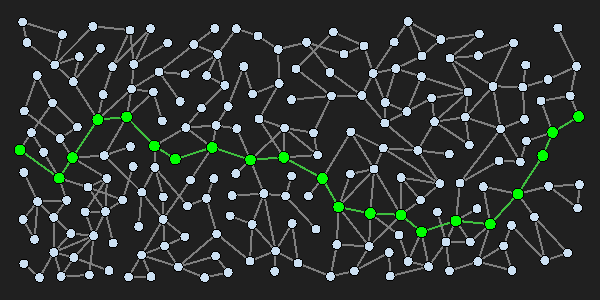
\includegraphics[width=0.75\linewidth]{images/graph-pathfinding.png}
                \caption{Beispiel für Pathfinding auf einem Graphen\\\cite{EZ:Web05}}
                \label{fig:graph-pathfinding}
            \end{figure}
        
    \section{Graphentheorie}

        Die Graphentheorie ist eines der wichtigsten Konzepte im Bereich des Pathfinding. Ein Graph ist eine abstrakte, mathematische Struktur, die aus Knoten und Kanten besteht. In Bezug auf Pathfinding repräsentieren die Knoten die Standorte oder Punkte, zwischen denen man Wege finden möchte, und die Kanten stellen die theoretisch möglichen oder tatsächlich vorhandenen Verbindungen zwischen diesen Punkten dar. Bei Navigationssystemen für die reale Welt, wie Google Maps, Waze und anderen, repräsentieren Kanten \zb Straßen und Knoten die Kreuzungen. \cite{EZ:Web03, EZ:Web06, EZ:Web29}

        \subsection{Visualisierung}
        
            In den meisten Fällen werden Knoten als Kreise oder Punkte dargestellt, oft auch mit einer zusätzlichen Beschriftung oder Bezeichnung. Die Kanten werden meist als einfache Linien zwischen den Knoten dargestellt, ist der Graph jedoch ein gerichteter, sind es Pfeile anstatt Linien. Ist er gewichtet, sind die einzelnen Gewichtungen meist neben den dazugehörigen Kanten aufzufinden. \cite{EZ:Web07}

        \subsection{Kantengewichtete Graphen} \label{kantengewichtete-graphen}

            Ein Graph $G = (V, E)$ wird als kantengewichtet bezeichnet, wenn jeder Kante $e \in E$ eine Gewichtung $w(e)$ zugeordnet wird, wobei $w: E \rightarrow \mathbb{R}$ beziehungsweise $w: V \times V \rightarrow \mathbb{R}$ die Kantengewichtungsfunktion ist. Die Gewichtungen der Kanten können abhängig vom Anwendungsfall unterschiedlich interpretiert werden. Meistens stellen sie die euklidische Distanz zwischen zwei Knoten dar, oftmals aber auch die benötigte Zeit, um vom einen Knoten zum anderen zu gelangen. Letzteres ist zum Beispiel bei der Routenplanung im Straßenverkehr nützlicher, da stockender Verkehr und Staus berücksichtigt werden können. Es gibt auch Graphen, die knotengewichtet sind, diese finden aber nur selten Verwendung. Da es für knotengewichtete Graphen weitaus weniger Anwendungsfälle gibt, als für kantengewichtete, werden kantengewichtete Graphen meist nur als gewichtet bezeichnet. \cite{EZ:Web04, EZ:Web10, EZ:Web22, EZ:Web32, EZ:Web35}
            
            Verläuft in einem gewichteten Graphen zwischen zwei Knoten $u$ und $v$ keine Kante, gilt
            
                \[w(u, v) = \infty\]
            
            weil ein Wert von $0$ eine Kante mit einer Gewichtung von $0$ implizieren würde, solche Kanten aber durchaus sinnvoll sein können. Für ungewichtete Graphen gilt eine spezielle Kantengewichtungsfunktion, die folgendermaßen definiert ist:

                \[
                    w(u, v) =   \begin{cases}
                                    1 & $falls u und v verbunden sind,$\\
                                    0 & $sonst.$
                                \end{cases}
                \]
            
            \abb{fig:weighted-graph} zeigt ein einfaches Beispiel für einen Graphen. Er besteht aus fünf Knoten und fünf Kanten, die Verbindungen zwischen den Knoten darstellen. Alle Knoten sind mit einzigartigen Buchstaben beschriftet, damit man sie eindeutig identifizieren kann. Die Zahlen neben den einzelnen Kanten sind deren jeweiligen Gewichtungen, was bedeutet, dass der gezeigte Graph ein gewichteter ist. \cite{EZ:Web42, EZ:Web43}
            
            \begin{figure}
                \centering
                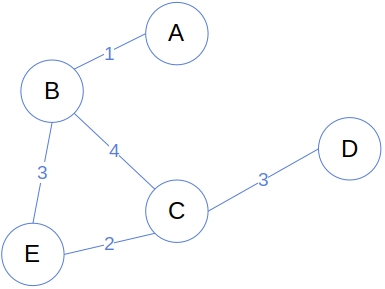
\includegraphics[width=0.5\linewidth]{images/weighted.jpg}
                \caption{Ein gewichteter Graph\\\cite{EZ:Web04}}
                \label{fig:weighted-graph}
            \end{figure}

        \subsection{Gerichtete Graphen} \label{gerichtete-graphen}

            Ein gerichteter Graph ist ein Graph, dessen Kanten nur in eine Richtung überquert werden dürfen. Wird eine ungerichtete Kante zwischen zwei Knoten benötigt, werden stattdessen zwei \emph{gegenläufige}, gerichtete Kanten verwendet. Gegenläufig oder \emph{antiparallel} nennt man zwei Kanten $e_1$, $e_2$ mit $e_1 = (a, b)$ und $e_2 = (b, a)$, wobei $a, b \in V$. Die Kanten eines gerichteten Graphen nennt man gerichtete Kanten und sind geordnete Knotenpaare $(a, b) \in E$ wobei man Kanten eines ungerichteten Graphen als ungerichtet bezeichnet werden und ungeordnete Knotenpaare $\{a, b\} \in E$ sind. Ein gerichteter Graph wird häufig auch als \emph{Digraph}\footnote{directed graph} bezeichnet. Ein Beispiel eines Digraphen ist in \abb{fig:digraph} zu sehen. \cite{EZ:Web20}

            \begin{figure}
                \centering
                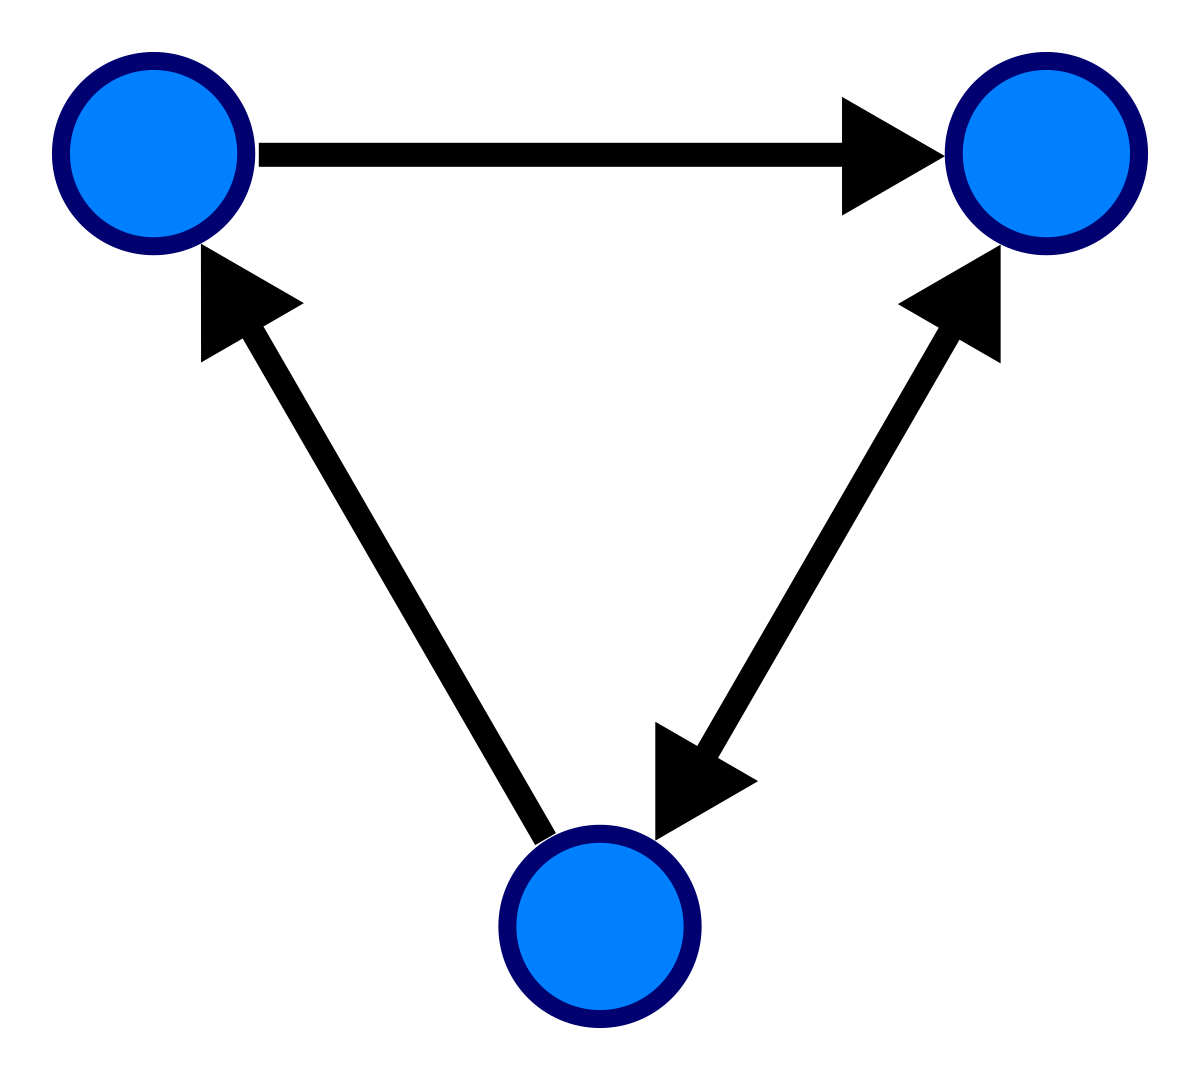
\includegraphics[width=0.4\linewidth]{images/digraph.png}
                \caption{Ein Digraph\\\cite{EZ:Web20}}
                \label{fig:digraph}
            \end{figure}
        
        \subsection{Multigraphen}

            Multigraphen sind Graphen, in denen sowohl \emph{Multikanten} als auch \emph{Schlingen} vorkommen dürfen. Als Multikanten oder Mehrfachkanten bezeichnet man mehrere gleichartige Kanten, die durch ein und dasselbe Knotenpaar verlaufen. Multikanten, die denselben Anfangs- und Endknoten haben, nennt man \emph{parallel}. Sind zwei Multikanten, die durch dieselben zwei Knoten verlaufen, gerichtet, und zeigen diese in entgegengesetzte Richtungen, werden sie als \emph{gegenläufig} oder \emph{antiparallel} bezeichnet, \skpt{gerichtete-graphen}. \cite{EZ:Web29, EZ:Web39}
            
            \emph{Schlingen} oder \emph{Schleifen} sind Kanten, die einen Knoten mit sich selbst verbinden. Ab hier wird in dieser Arbeit ausschließlich der Begriff \emph{Schlinge} verwendet, um Verwechslungen mit Schleifen aus der Programmierung zu vermeiden. \abb{fig:loop} veranschaulicht einen Multigraphen mit einer Schlinge. In den Abbildungen \ref{fig:multi-edge-directed} und \ref{fig:multi-edge-undirected} sind gerichtete beziehungsweise ungerichtete Multigraphen visualisiert. \cite{EZ:Web27, EZ:Web28, EZ:Web39}

            \begin{figure}
                \centering
                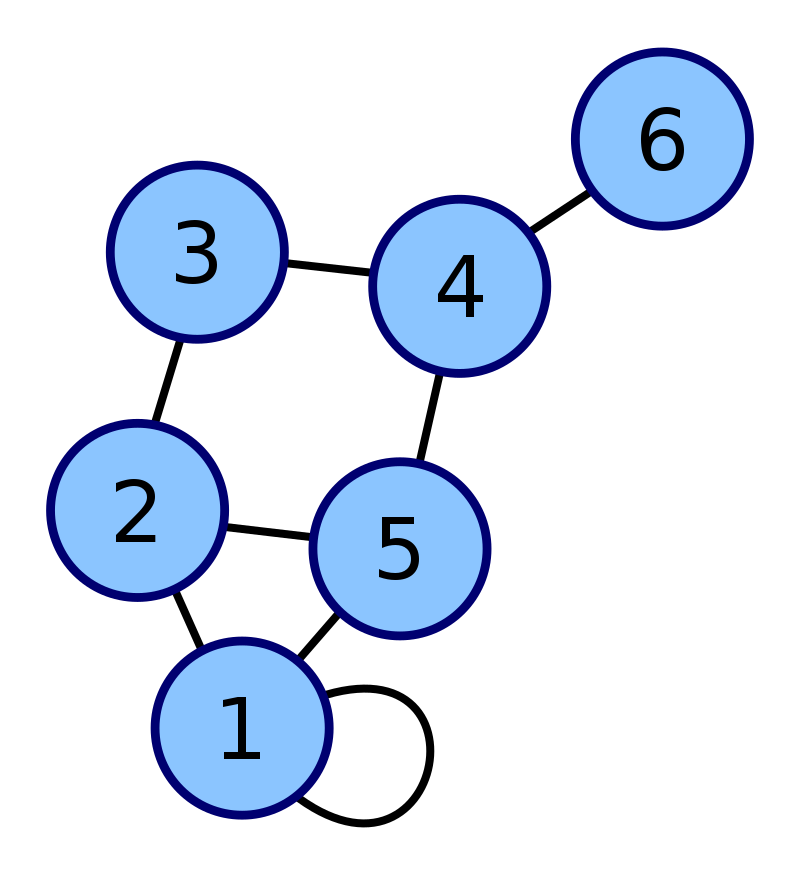
\includegraphics[width=0.4\linewidth]{images/loop.png}
                \caption{Ein Multigraph mit einer Schlinge\\\cite{EZ:Web27, EZ:Web28}}
                \label{fig:loop}
            \end{figure}

            \begin{figure}
                \centering
                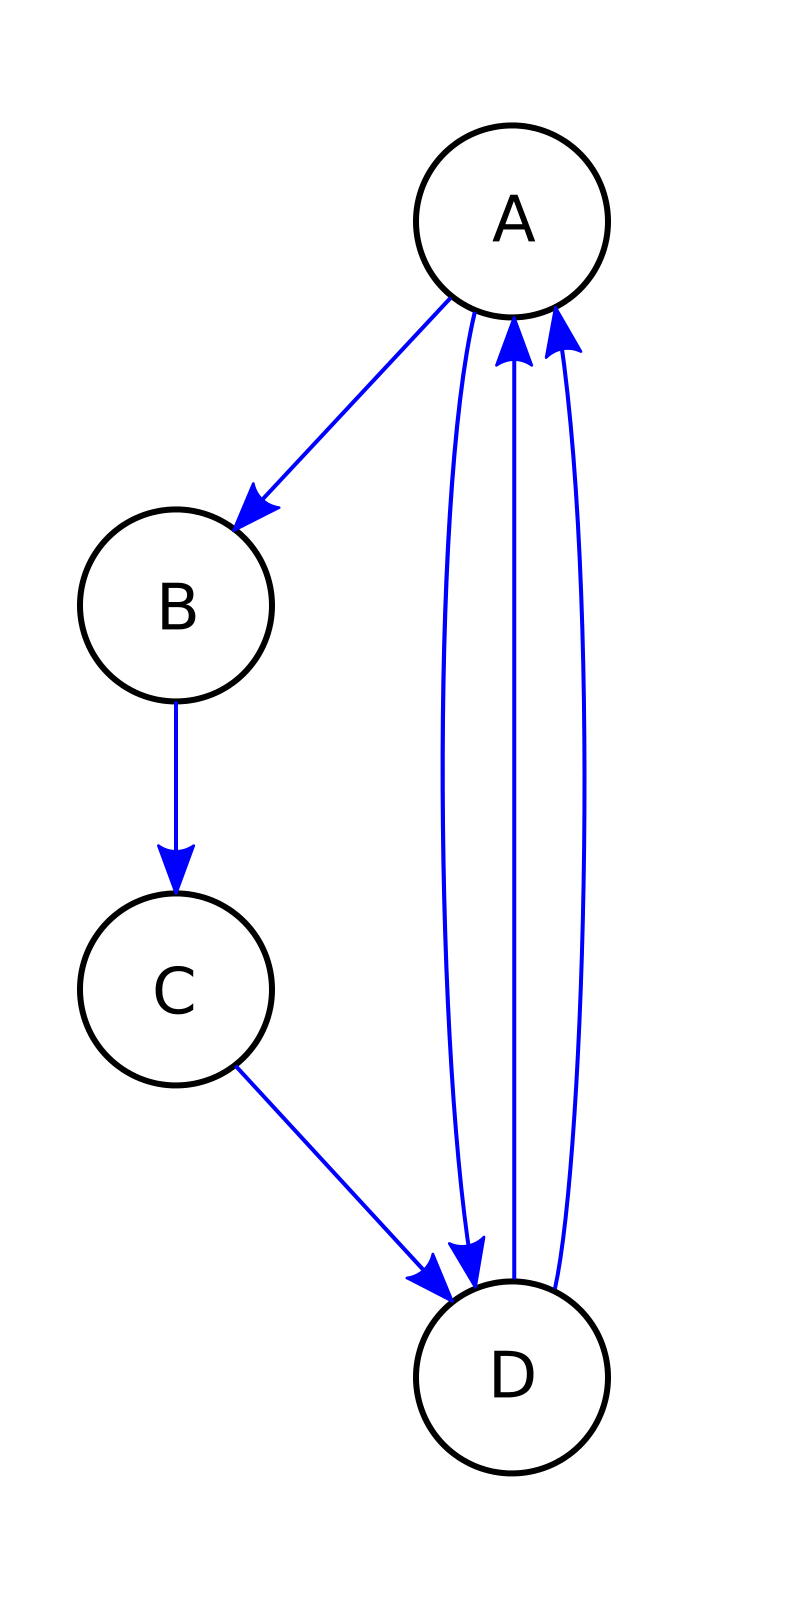
\includegraphics[width=0.25\linewidth]{images/multi-edge-directed.png}
                \caption{Ein gerichteter Graph mit Multikanten\\\cite{EZ:Web29}}
                \label{fig:multi-edge-directed}
            \end{figure}

            \begin{figure}
                \centering
                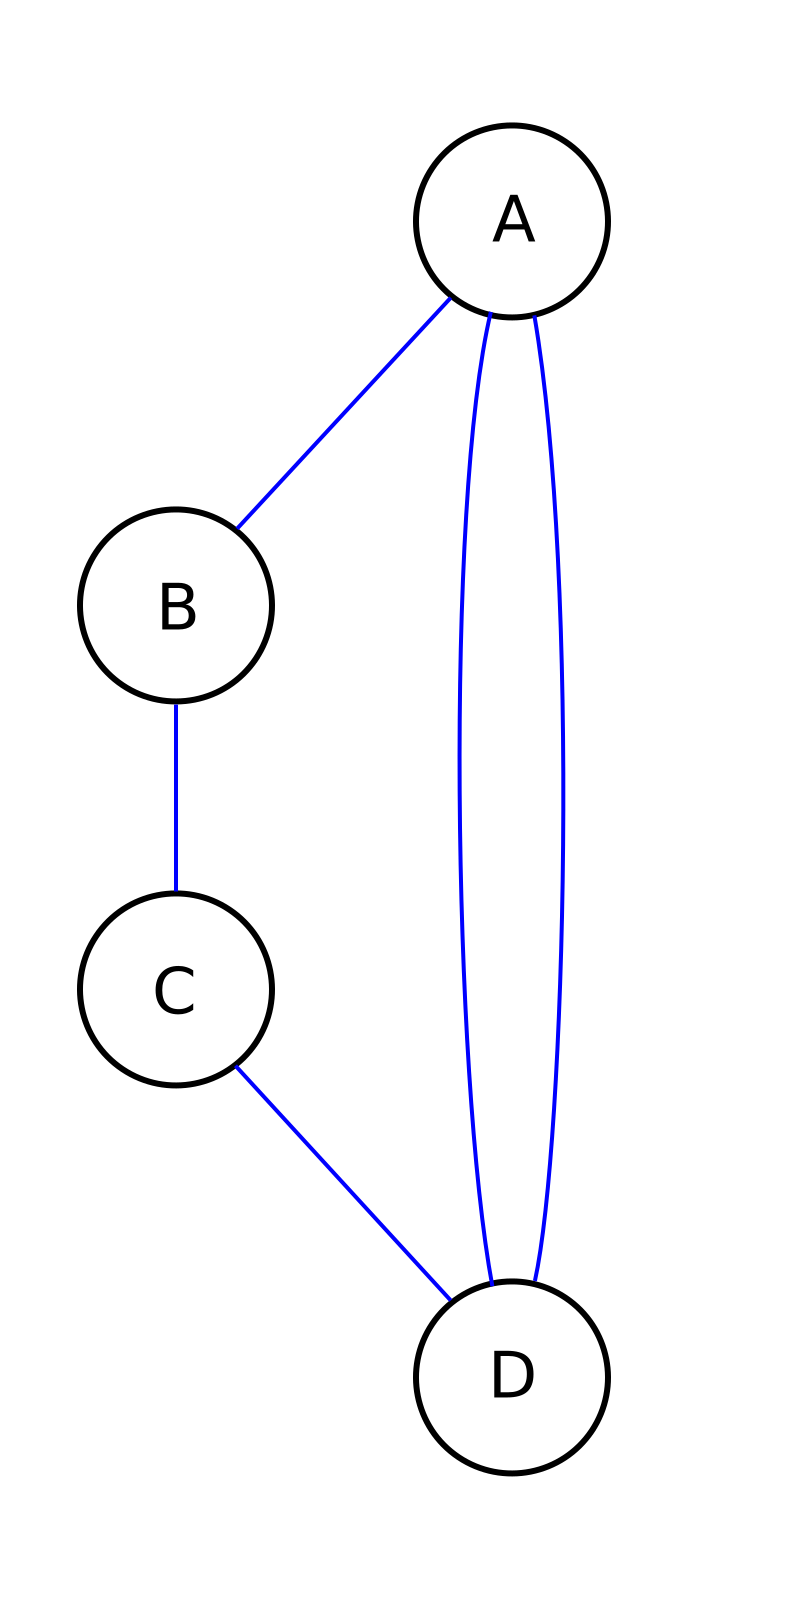
\includegraphics[width=0.25\linewidth]{images/multi-edge-undirected.png}
                \caption{Ein ungerichteter Graph mit Multikanten\\\cite{EZ:Web29}}
                \label{fig:multi-edge-undirected}
            \end{figure}
        
        \subsection{Einfache Graphen}

            Im Unterschied zu Multigraphen bezeichnet man Graphen, die ungerichtet sind und weder Multikanten noch Schlingen aufweisen, als \emph{einfach} oder \emph{schlicht}. In \abb{fig:graph} ist ein Beispiel eines einfachen Graphen zu sehen. \cite{EZ:Web26}

            \begin{figure}
                \centering
                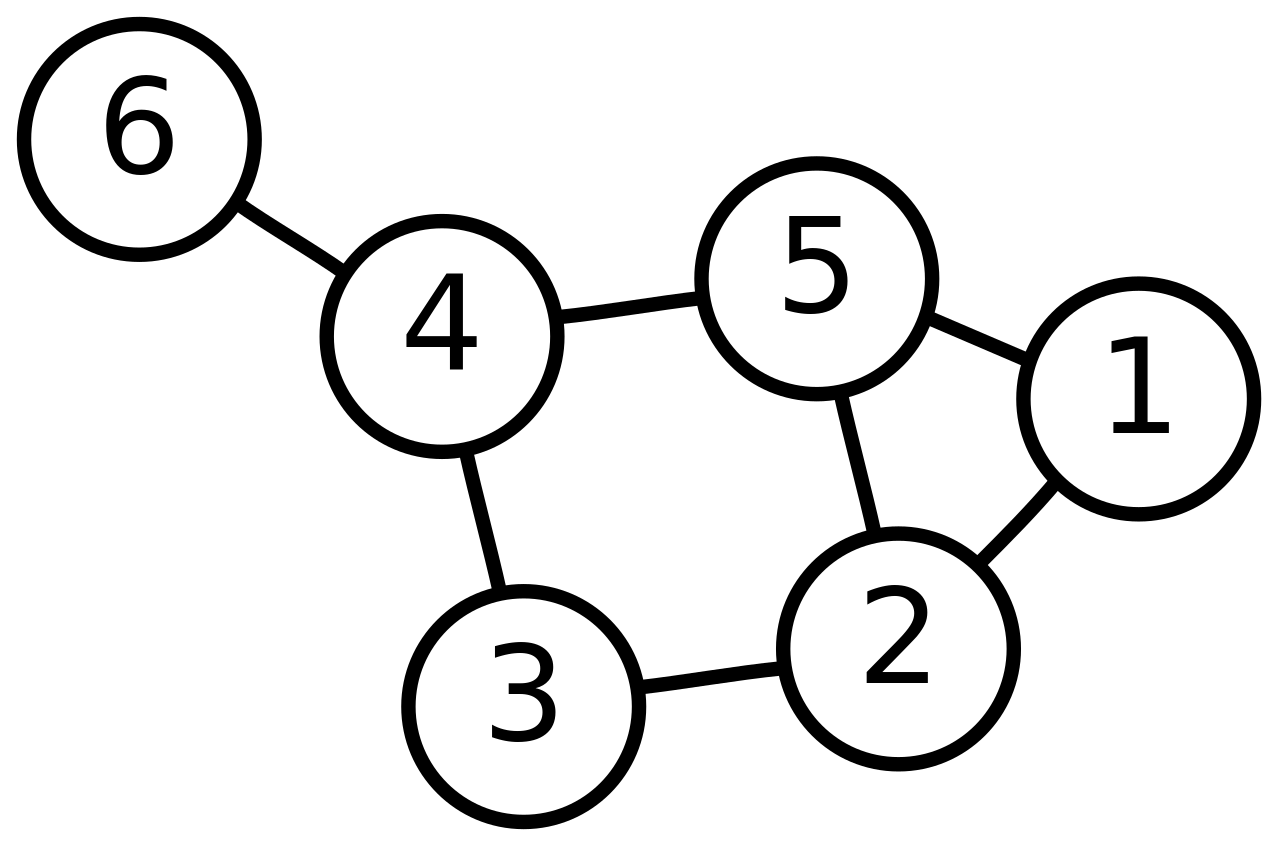
\includegraphics[width=0.5\linewidth]{images/graph.png}
                \caption{Ein einfacher Graph mit sechs Knoten und sieben Kanten\\\cite{EZ:Web25}}
                \label{fig:graph}
            \end{figure}

        \subsection{Netzwerke}
            
            Ist ein Graph sowohl gewichtet als auch gerichtet, ist er also ein gewichteter Digraph, spricht man von einem Netzwerk. Die Definition ist jedoch nicht einheitlich, zum Beispiel sind umgangssprachlich oft nur gewichtete Graphen oder gar Graphen im Allgemeinen gemeint, wenn von Netzwerken die Rede ist. In \abb{fig:network} ist ein Netzwerk mit fünf nummerierten Knoten und sieben Kanten zu sehen. \cite{EZ:Web09, EZ:Web25}
            
            \begin{figure}
                \centering
                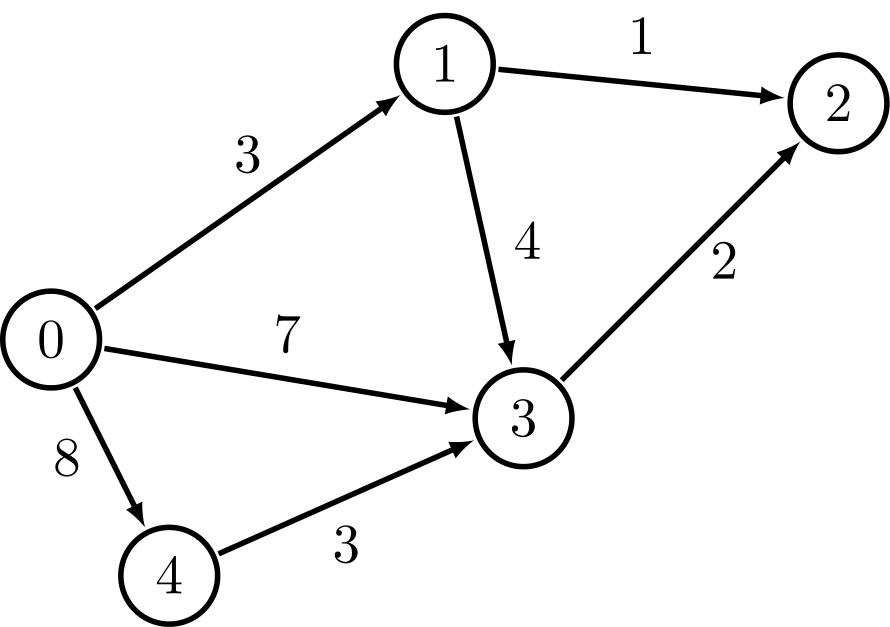
\includegraphics[width=0.5\linewidth]{images/network.png}
                \caption{Ein Netzwerk\\\cite{EZ:Web10}}
                \label{fig:network}
            \end{figure}

        \subsection{Symbolik}

            In den kommenden Abschnitten werden einige Symbole der Mengenlehre und Prädikatenlogik eingesetzt. Um klarzustellen, was diese bedeuten, sind die Definitionen der wichtigsten davon in \tbl{tab:symbols} auf Deutsch und auf Englisch aufzufinden.

            \begin{table}
                \centering
                \begin{tabular}{|c|l|l|} \hline
                    Symbol & Bedeutung & Meaning\\ \hline
                    $\{\ldots\}$ & Menge & set\\
                    $|\ldots|$ & Kardinalität (Mächtigkeit) & cardinality\\
                    $\in$ & Element von & element of\\
                    $\notin$ & kein Element von & not element of\\
                    $\exists$ & es existert mindestens ein & there exists at least one\\
                    $\exists!$ & es existiert genau ein & there exists one and only one\\
                    $\forall$ & für alle & for all\\ \hline
                \end{tabular}
                \caption{Wichtige Symbole der Mengenlehre\\\cite{EZ:Web23, EZ:Web24}}
                \label{tab:symbols}
            \end{table}

        \subsection{Zyklen}

            Ein Graph $G = (V, E)$ ist genau dann zyklisch, wenn seine Kanten mindestens einen \emph{Zyklus} bilden. Ein Zyklus ist eine Teilmenge der Kantenmenge $E$ eines Graphen, die einen Pfad formt, sodass der erste Knoten des Pfades dem letzten entspricht. Einen Zyklus in einem gerichteten Graphen bezeichnet man als gerichteten Zyklus und einen Zyklus in einem ungerichteten Graphen als ungerichteten Zyklus. Für einen ungerichteten Zyklus der \emph{Länge} $k \in \mathbb{N}$ mit der Knotenfolge $(v_1, v_2, \ldots, v_k, v_1)$  gilt somit $\forall i \in \{1, 2, \ldots, k\} \exists e_i$ wobei $e_i = \{v_i, v_{i+1}\} \in E$ eine Kante ist, die $v_i$ mit $v_{i+1}$ verbindet und $v_{k+1} = v_1$. Somit sind $v_{k}$ und $v_{k+1}$ miteinander verbunden, was impliziert, dass $v_{k}$ mit $v_1$ verbunden ist und sich somit ein Zyklus bildet. \cite{EZ:Web11, EZ:Web12}
            
            Obiges gilt auch für gerichtete Zyklen, jedoch ist die Länge dort oft nicht, wie bei ungerichteten Zyklen, als die Anzahl der Knoten oder Kanten, aus denen der Zyklus besteht, definiert, sondern als die Summe der Gewichtungen der im Zyklus überquerten Kanten. \cite{EZ:Web16, EZ:Web17}

        \subsection{Kreise}
        
            Ein \emph{Kreis} ist eine Sonderform eines Zyklus, bei dem der Pfad ein einfacher ist, also sind nicht nur die überquerten Kanten des Pfades einzigartig, sondern auch die überquerten Knoten. Somit müssen sich die Knoten $v_1, v_2, \ldots, v_k$ alle voneinander unterscheiden. \abb{fig:cyclic-graph} zeigt ein simples Beispiel eines zyklischen Graphen, dessen Zyklus ein Kreis ist. \cite{EZ:Web13}

            \begin{figure}
                \centering
                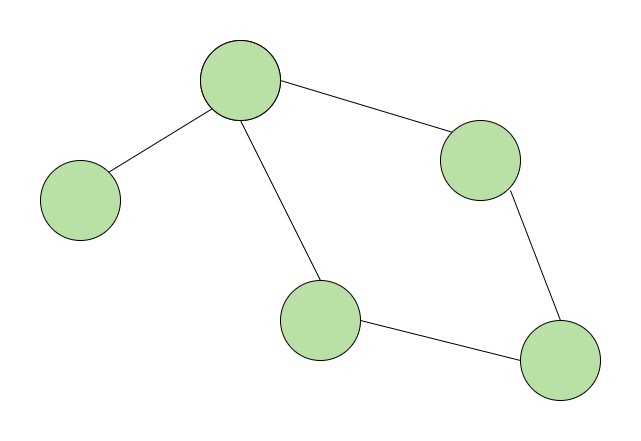
\includegraphics[width=0.5\linewidth]{images/cyclic-graph.png}
                \caption{Ein zyklischer Graph mit einem Kreis\\\cite{EZ:Web12}}
                \label{fig:cyclic-graph}
            \end{figure}

        \subsection{Kreisgraphen}

            Enthält ein Graph genau einen Zyklus, welcher gleichzeitig ein Kreis ist, und besteht dieser aus der gesamten Knotenmenge $V$ des Graphen, bezeichnet man den Graphen als \emph{Kreisgraph}. Für einen Kreisgraphen gilt immer
            
                \[|V| = |E|\]
            
            was bedeutet, dass die Anzahl der Knoten mit der der Kanten übereinstimmt. Die ersten fünf Kreisgraphen $C_1$, $C_2$, $C_3$, $C_4$ und $C_5$ sind in \abb{fig:cycle-graphs} veranschaulicht. Der Knoten des Kreisgraphen $C_1$ ist durch eine Schlinge mit sich selbst verbunden. \cite{EZ:Web14, EZ:Web15}

            \begin{figure}
                \centering
                \includesvg[width=0.75\linewidth]{images/cycle-graphs.svg}
                \caption{Die Kreisgraphen $C_1$, $C_2$, $C_3$, $C_4$ und $C_5$\\\cite{EZ:Web14}}
                \label{fig:cycle-graphs}
            \end{figure}

        \subsection{Vollständige Graphen}
        
            Ein vollständiger Graph ist ein einfacher Graph, in dem jeder Knoten eine Kante zu allen anderen im Graphen enthaltenen Knoten hat. Anders ausgedrückt: Jedes Paar von unterschiedlichen Knoten ist durch eine Kante verbunden. Für einen \emph{vollständigen Digraphen} gilt ähnlich: Jedes Paar von unterschiedlichen Knoten ist durch \textit{ein Paar von unterschiedlichen Kanten} verbunden, also mit einer Kante je Richtung. In \abb{fig:complete-graphs} sind die vollständigen Graphen $K_1$, $K_2$, $K_3$, $K_4$ und $K_5$ zu sehen. \cite{EZ:Web33, EZ:Web34}

            \begin{figure}
                \centering
                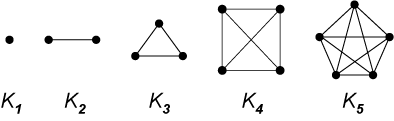
\includegraphics[width=0.5\linewidth]{images/complete-graphs.png}
                \caption{Die vollständigen Graphen $K_1$, $K_2$, $K_3$, $K_4$ und $K_5$\\\cite{EZ:Web33}}
                \label{fig:complete-graphs}
            \end{figure}

        \subsection{Bipartite Graphen}

            Ein Graph ist \emph{bipartit}, wenn eine der beiden folgenden Aussagen gilt:

            \begin{itemize}
                \item Der Graph ist azyklisch

                \item Für jeden Zyklus mit der Knotenfolge $(v_1, v_2, \ldots, v_n, v_1) \in V$ gilt $n \equiv 0 \pmod{2}$. Es gilt also für keinen Zyklus $n \equiv 1 \pmod{2}$.
            \end{itemize}
            
            Ist ein Graph bipartit, kann man seine Knoten in zwei disjunkte Teilmengen aufteilen, sodass zwischen den Knoten innerhalb beider Teilmengen keine Kanten verlaufen. Damit das Ganze etwas greifbarer ist, ist die genannte Bedingung in \abb{fig:bipartite-graph} mithilfe eines Beispiels für solch einen Graphen verdeutlicht. Der gezeigte Graph ist nicht \emph{vollständig bipartit}, da nicht jeder Knoten der Teilmenge $U$ eine Kante zu jedem Knoten der Teilmenge $V$ hat. Ein Beispiel für einen Graphen, der diese Bedingung erfüllt und somit vollständig bipartit ist, ist in \abb{fig:complete-bipartite-graph} veranschaulicht. \cite{EZ:Web12, EZ:Web19}

            \begin{figure}
                \centering
                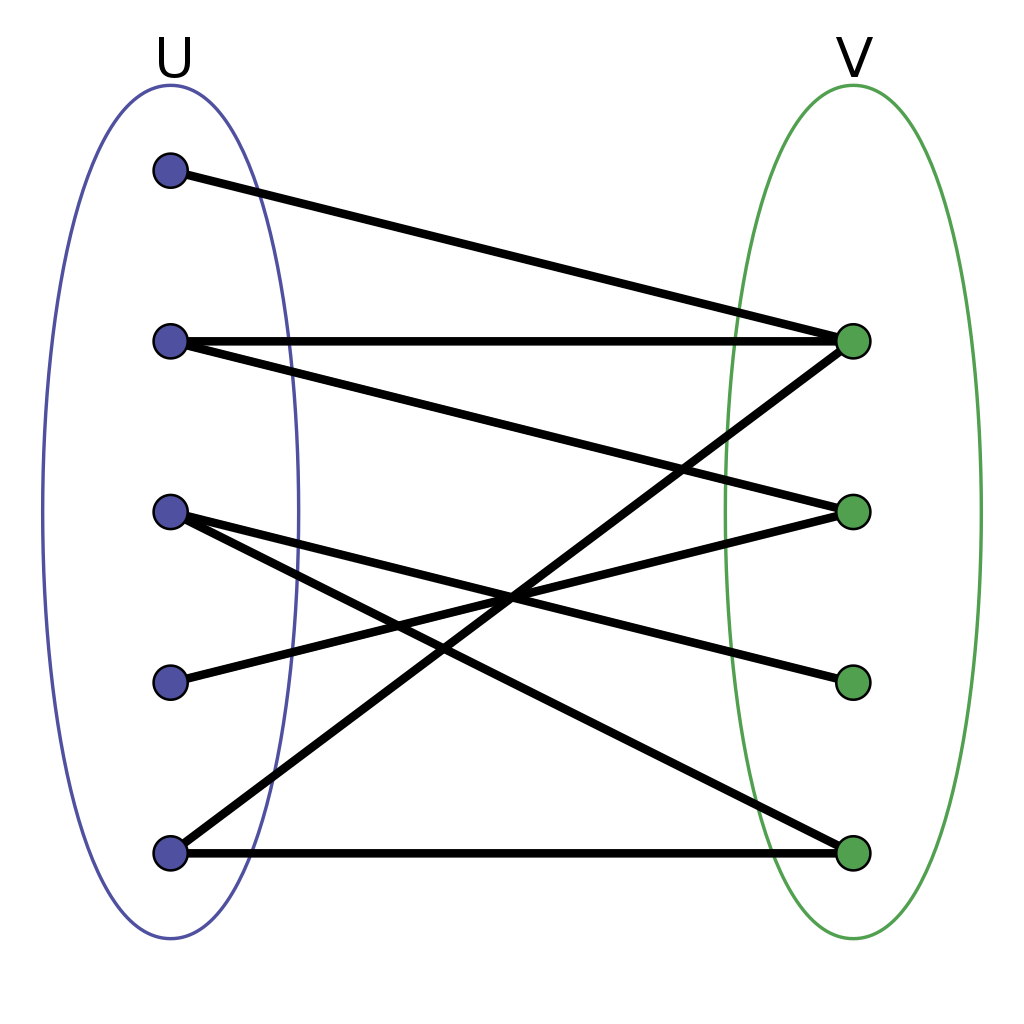
\includegraphics[width=0.4\linewidth]{images/bipartite-graph.png}
                \caption{Ein einfacher, nicht vollständig bipartiter Graph mit Partitionsklassen $U$ und $V$\\\cite{EZ:Web19}}
                \label{fig:bipartite-graph}
            \end{figure}

            \begin{figure}
                \centering
                
\includegraphics[width=0.3\linewidth]{images/complete-bipartite-graph.png}
                \caption{Ein einfacher, vollständig bipartiter Graph\\\cite{EZ:Web19}}
                \label{fig:complete-bipartite-graph}
            \end{figure}

        \subsection{Grids}

            Neben Graphen werden für Pathfinding häufig auch Grids verwendet, da diese für einige Anwendungsfälle besser geeignet sind, da es keine vordefinierten Kanten gibt. Ein Grid kann als Sonderfall eines Graphen betrachtet werden, bei dem die Knoten in gleichmäßigen Abständen platziert sind und jeder Knoten Kanten zu allen Knoten hat, die ihn umgeben, sofern diese nicht von Hindernissen oder Ähnlichem blockiert sind. Ein Beispiel für Pathfinding auf einem Grid ist in \abb{fig:grid-pathfinding} zu sehen. Hier ist der rote Kreis der Startpunkt und der grüne der Zielpunkt. Die dunklen Zellen stellen Hindernisse dar, die der Pfad vermeiden muss. In diesem spezifischen Fall sind diagonale Schritte erlaubt, weshalb der kürzeste Weg zwei Diagonalen beinhaltet. Stellt man das Grid als Graph dar, existieren entweder keine Kanten zu den blockierten Knoten oder die Hindernisse werden erst gar nicht als Knoten dargestellt, sondern schlicht und ergreifend verworfen.

            \begin{figure}
                \centering
                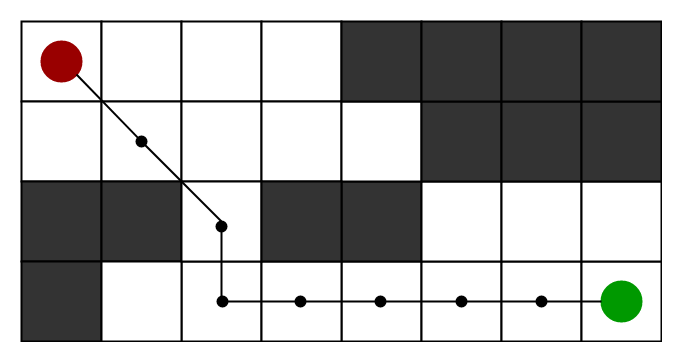
\includegraphics[width=0.5\linewidth]{images/grid-pathfinding.png}
                \caption{Beispiel für Pathfinding auf einem Grid\\\cite{EZ:Web02}}
                \label{fig:grid-pathfinding}
            \end{figure}

        \subsection{Darstellung} \label{darstellung}

            \subsubsection{Adjazenzliste}

                Mithilfe einer \emph{Adjazenzliste} kann ein Graph mitsamt dessen Knoten und Kanten dargestellt werden. Sie ist eine einfache Auflistung aller Nachbarknoten für jeden Knoten, wobei mit Nachbarknoten alle Knoten gemeint sind, zu denen ein Knoten eine Kante hat. Will man einen gewichteten Graphen als Adjazenzliste darstellen, speichert man gemeinsam mit jeder Kante ihre zugehörige Gewichtung ab. Adjazenzlisten eignen sich gut für gerichtete Graphen, da man mit ihnen nur die von Knoten \textit{ausgehenden} Kanten beschreibt, nicht die eingehenden. Für ungerichtete Graphen ergeben sich somit zwei Möglichkeiten sie als Adjazenzliste abzuspeichern:

                \begin{enumerate}
                    \item Man speichert jede ungerichtete Kante $\{v_i, v_j\}$ als zwei gegenläufige gerichtete Kanten ab: bei Knoten $v_i$ als $(v_i, v_j)$ und bei Knoten $v_j$ als $(v_j, v_i)$. Dadurch ist es egal, auf welcher Seite man auf die Existenz einer Kante prüft. Ein Vorteil dieser Methode ist, dass man garantiert immer nur einen Kanten-Check durchführen muss und man deshalb auch nicht klarstellen muss, ob es sich um einen gerichteten oder einen ungerichteten Graphen handelt, solange man den Graphen nicht mehr verändert. Man kann bei Anwendung dieser Methode eine Art Mischung aus einem gerichteten und einem ungerichteten Graphen darstellen, da gerichtete Kanten nur bei ihrem Startknoten abgespeichert werden müssen. Der klare Nachteil ist der doppelte Speicherverbrauch für ungerichtete Kanten.

                    \item Man speichert jede ungerichtete Kante $\{v_i, v_j\}$  nur einmal ab, entweder bei $v_i$ oder bei $v_j$, wodurch weniger Speicherplatz beansprucht wird. Prüft man jedoch von Knoten $v_i$ ausgehend, ob zum Knoten $v_j$ eine Kante $(v_i, v_j)$ existiert und stellt fest, dass das nicht der Fall ist, so muss auch auf die Existenz der gegenläufigen Kante $(v_j, v_i)$ geprüft werden. Geht man davon aus, dass man in durchschnittlich $50 \%$ der Fälle vom Startknoten und in $50 \%$ der Fälle vom Endknoten der zu überprüfenden Kante ausgehend prüft, so müssen in der Hälfte aller Fälle zwei Checks durchgeführt werden, was bedeutet, dass durchschnittlich $0.5 \cdot 1 + 0.5 \cdot 2 = 1.5$ Checks durchgeführt werden müssen, was ein klarer Nachteil ist. Damit die Existenz der gegenläufigen Kante $(v_j, v_i)$ auch wirklich geprüft wird, falls $(v_i, v_j)$ nicht existiert, muss klargestellt werden, dass es sich um einen ungerichteten Graphen handelt. Durch diesen Nachteil ergibt sich auch schon der nächste: Es gibt bei dieser Methode keine Möglichkeit, gerichtete Kanten darzustellen, sie kann also nur bei rein ungerichteten Graphen eingesetzt werden.
                \end{enumerate}
                
                \tbl{tab:adjacency-list} stellt die Adjazenzliste für den Graphen, der in \abb{fig:triangle} zu sehen ist, dar. Der verwendete Graph ist ungerichtet und zur Darstellung wird Methode 1 angewendet. \cite{EZ:Web31, EZ:Web40}
    
                \begin{figure}
                    \centering
                    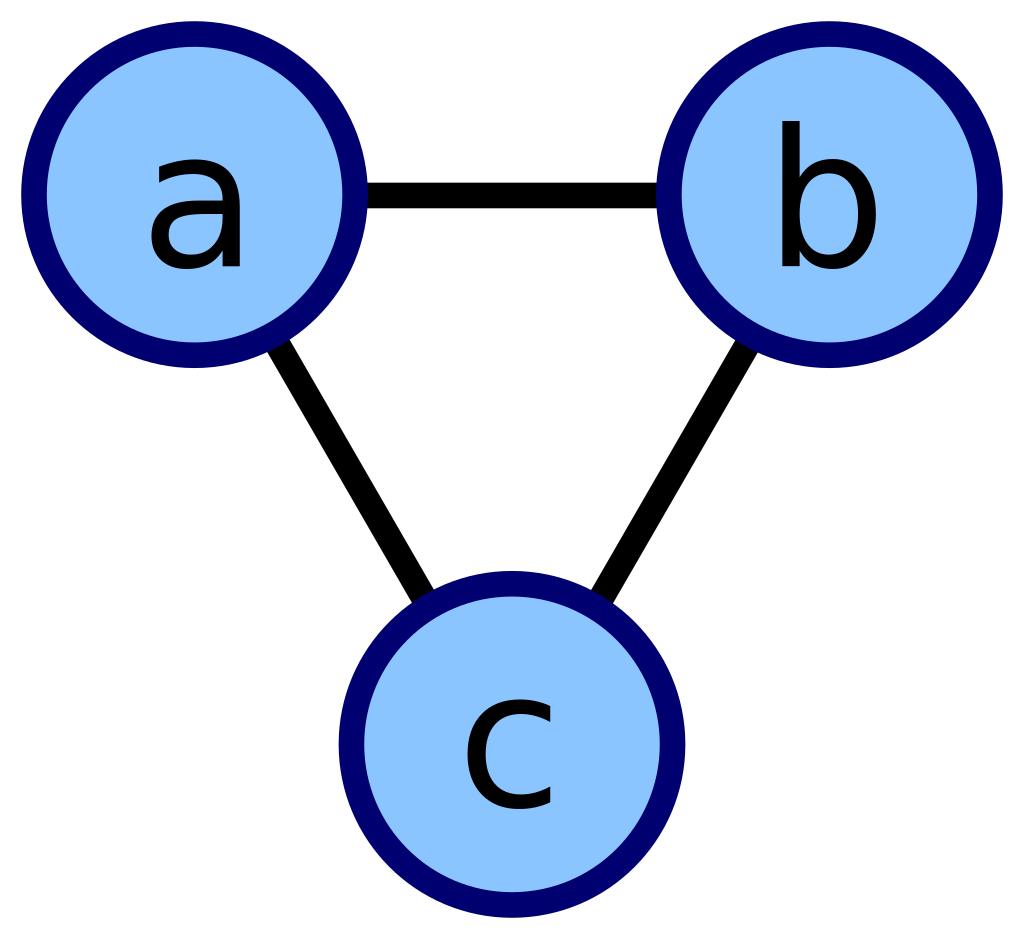
\includegraphics[width=0.25\linewidth]{images/graph-adjacency.png}
                    \caption{$C_3$ beziehungsweise $K_3$, der kleinste Dreiecksgraph\\\cite{EZ:Web31}}
                    \label{fig:triangle}
                \end{figure}
                
                \begin{table}
                    \centering
                    \begin{tabular}{c|c}
                         Knoten & adjazent mit\\ \hline
                         a & b, c\\
                         b & a, c\\
                         c & a, b\\
                    \end{tabular}
                    \caption{Adjazenzliste}
                    \label{tab:adjacency-list}
                \end{table}
                
            \subsubsection{Adjazenzmatrix}
    
                \emph{Adjazenzmatrizen} bieten eine weitere Möglichkeit, einen Graphen $G = (V, E)$ darzustellen. Eine Adjazenzmatrix $A$ ist eine quadratische $|V| \times |V|$-Matrix. Sie speichert in jedem Element $A_{i,j}$ die Gewichtung der Kante zwischen den Knoten $v_i$ und $v_j$. Wird sie an einem ungewichteten Graphen angewandt, wird eine $1$ gespeichert, falls es eine Kante zwischen den beiden Knoten gibt. Verläuft keine Kante durch $v_i$ und $v_j$, speichert sie den Wert $0$ oder $\infty$. Für gewichtete Graphen eignet sich $\infty$ besser, da $0$ in manchen Fällen eine sinnvolle Gewichtung für Kanten sein kann. Adjazenzmatrizen haben den Vorteil, dass sie übersichtlich und, wie Adjazenzlisten, gut für gerichtete Graphen geeignet sind. Ihr großer Nachteil ist jedoch, dass es viele redundante Werte gibt, da Kanten, die nicht existieren, nicht abgespeichert werden müssten. Adjazenzmatrizen haben im Durchschnittsfall eine quadratische Platzkomplexität, wie in \tbl{tab:adjacency-space-complexities} angeführt. Aus diesem Grund sind Adjazenzmatrizen nur für eher kleine Graphen geeignet. In \tbl{tab:adjacency-matrix} ist die Adjazenzmatrix für den Graphen aus \abb{fig:triangle} zu sehen. \cite{EZ:Web36, EZ:Web37, EZ:Web41, EZ:Web42, EZ:Web43}
                
                \begin{table}
                    \centering
                    \begin{tabular}{|l|l|l|} \hline 
                        \textbf{Case} & \textbf{Adjazenzliste} & \textbf{Adjazenzmatrix}\\ \hline
                        Average & $\bigO(|V| + |E|)$ & $\bigO(|V|^2)$\\
                        Worst & $\bigO(|V|^2)$ & $\bigO(|V|^2)$\\ \hline
                        
                    \end{tabular}
                    \caption{Die Platzkomplexitäten der Adjazenzliste und -matrix\\\cite{EZ:Web40}}
                    \label{tab:adjacency-space-complexities}
                \end{table}
                
                \begin{table}
                    \centering
                    \begin{tabular}{c|ccc}
                          & a & b & c\\ \hline 
                        a & 0 & 1 & 1\\
                        b & 1 & 0 & 1\\
                        c & 1 & 1 & 0\\
                    \end{tabular}
                    \caption{Adjazenzmatrix des Graphen aus \abb{fig:triangle}}
                    \label{tab:adjacency-matrix}
                \end{table}

        \subsection{Implementierung}

            Für fertige Implementierungen gibt es zahlreiche Libraries, wie \zb \emph{NetworkX} für Python oder \emph{JGraphT} für Java. Um jedoch zu verstehen, wie diese intern funktionieren, wird das Konzept eines Graphen in dieser Arbeit von Grund auf neu implementiert: In \lil{lst:graph-interface} wird das generische Interface \lstinline{Graph<T>} definiert, welches dazu dient, mehrere unterschiedliche Arten von Graphen darstellen zu können, zum Beispiel auch unendlich große. Das Interface schreibt genau eine Methode vor, die implementiert werden muss: \lstinline{Map<T, Double> getNeighbors(T vertex)}. Mithilfe von dieser können alle Nachbarn eines gegebenen Knoten inklusive der Gewichtungen der Kanten zu diesen berechnet werden. Dadurch können auch unendlich große Graphen dargestellt werden, da die tatsächliche Struktur des Graphen nicht abgespeichert werden muss, sondern durch seine Adjazenzen impliziert werden kann. Zusätzlich sind \lstinline{double hasEdge(T source, T destination)}, \lstinline{int getDegree(T vertex)}, \lstinline{double getEdgeWeight(T source, T destination)} und \lstinline{double sumEdgeWeights(List<T> path)} defaultmäßig so implementiert, dass \lstinline{getNeighbors} in den Methoden \lstinline{hasEdge}, \lstinline{getDegree} und \lstinline{getEdgeWeight} zum Einsatz kommt und \lstinline{getEdgeWeight} wiederum in \lstinline{sumEdgeWeights} verwendet wird. Hierbei gibt \lstinline{hasEdge} einen \lstinline{boolean} zurück, der angibt, ob zwischen den beiden übergebenen Knoten in der angegeben Reihenfolge eine Kante verläuft. Mithilfe von \lstinline{int getDegree(T vertex)} kann man die Anzahl an Nachbarn des übergebenen Knotens erhalten. \lstinline{getEdgeWeight} ist dafür zuständig, die Gewichtung der Kante zurückzugeben, die zwischen den beiden übergebenen Knoten verläuft, bzw. $\infty$, falls die Knoten nicht (in der übergebenen Reihenfolge) miteinander verbunden sind. Die \lstinline{sumEdgeWeights}-Methode ist dazu da, die Gesamtgewichtung eines Pfades zu berechnen, was für manche Pathfinding-Algorithmen entscheidend ist.

            \lstinputlisting[
                caption=\texttt{Graph.java},
                label=lst:graph-interface
            ]{sources/Graph.java}

            Das Interface \lstinline{ModifiableGraph<T>} aus \lil{lst:modifiable-graph} ist eine Erweiterung von \lstinline{Graph<T>}, das einige zusätzliche Methoden vorschreibt. Mit diesen können Graph-Instanzen von Klassen, die dieses Interface implementieren, modifiziert werden und es können viele wichtige Informationen über sie ausgelesen werden. Beispielsweise kann mit \lstinline{double calculateAverageDegree()} die durchschnittliche Nachbaranzahl pro Knoten berechnet werden.

            \lstinputlisting[
                caption=\texttt{ModifiableGraph.java},
                label=lst:modifiable-graph
            ]{sources/ModifiableGraph.java}
            
            Eine simple, konkrete Graph-Klasse könnte in Java in etwa wie in \lil{lst:flexible-graph} aussehen. Sie implementiert das eben erwähnte \lstinline{Graph<T>}-Interface und ist generisch, da Graphen eine Unzahl an Anwendungsfällen haben. Zum Beispiel können neben Straßennetzen und vielem mehr auch Freundschaften in einem sozialen Netzwerk dargestellt und analysiert werden. In diesem Fall könnte man für den Typparameter \lstinline{T} beispielsweise eine \lstinline{Person} verwenden, oder \lstinline{String} für den Namen. Sind die Namen der Personen nicht eindeutig, können Klassen wie \lstinline{Integer}, \lstinline{Long} oder \lstinline{UUID} als Identifikator verwendet werden. \cite{EZ:Web21, EZ:Web45, EZ:Web46}
    
            In der Variable \lstinline{Map<T, Map<T, Double>> adjacencies} werden sowohl die Knoten als auch die von ihnen ausgehenden Kanten gespeichert, indem jedem Knotenwert in einer Map eine weitere Map zugeordnet wird, die jedem Nachbarn des Knotens, zu dem die (innere) Map gehört, die Gewichtungen der jeweiligen Kanten als \lstinline{Double} zuordnet. Der soeben beschriebene Ansatz, einen Graphen zu speichern, ist eine Form der in \kpt{darstellung} beschriebenen Adjazenzliste, mit dem lediglichen Zusatz der Kantengewichtungen. Für eine Implementierung eines ungewichteten Graphen wäre eine \lstinline{Map<T, List<T>>} völlig ausreichend, jedoch ist der Zweck dieser Klasse, möglichst viele Arten von Graphen darstellen zu können, daher auch der Name \lstinline{FlexibleGraph<T>}.

            Die Klasse ist mit einigen Lombok-Annotations ausgestattet, wie \zb \lstinline{@ToString} über der Klassendefinition für die automatische Generierung einer \lstinline{toString}-Methode, die einen \lstinline{String} zurückgibt, der den Namen der Klasse sowie sämtliche Instanzvariablennamen und -werte von dieser enthält. Außerdem ist sie mit \lstinline{@Getter} und \lstinline{@Setter} annotiert, damit für die \lstinline{final} Variablen \lstinline{boolean directed} und \lstinline{Map<T, Map<T, Double>> adjacencies} automatisch Getter mit den Namen \lstinline{isDirected} und \lstinline{getAdjacencies} erstellt werden und für die \lstinline{ToDoubleBiFunction<T, T> defaultWeightFunction} sowohl Getter als auch Setter erstellt werden. Bis auf den einzigen Unterschied, dass \lstinline{ToDoubleBiFunction::<T, U>applyAsDouble} einen primitiven \lstinline{double}, \lstinline{BiFunction::<T, U, Double>apply} hingegen den Wrapper \lstinline{Double} zurückgibt, sind die beiden Interfaces identisch. So wird dem Computer mit dem Einsatz von \lstinline{ToDoubleBiFunction} ein wenig Arbeit erspart, da der Rechenaufwand von Boxing und Unboxing wegfällt.
            
            Dem Konstruktor des Graphen wird ein \lstinline{boolean directed} übergeben, der angibt, ob der Graph gerichtet ist, oder nicht. Ist er ungerichtet, wird für jede hinzugefügte Kante eine gegenläufige Kante, also mit \lstinline{source} und \lstinline{destination} vertauscht, abgespeichert. Es kommt also die erste der beiden in \kpt{darstellung} genannten Möglichkeiten zur Darstellung für ungerichtete Graphen als Adjazenzliste zum Einsatz. Graphen wie diese können als eine Art gewichtete Adjazenzliste dargestellt werden. Ein Beispiel dafür ist in \tbl{tab:example-adjacency-list} zu sehen.

            \begin{table}
                \centering
                \begin{tabular}{c|l}
                    Knoten & Adjazenzen\\ \hline
                    A & B=1\\
                    B & C=3\\
                    C & E=7\\
                    D & A=8, C=1\\
                    E & A=5, B=3, C=2, D=5
                \end{tabular}
                \caption{Gewichtete Adjazenzliste des generierten Graphen aus \lil{lst:modifiable-graph-randomizer-example}}
                \label{tab:example-adjacency-list}
            \end{table}
            
            Wird der Parameter \lstinline{double weight} der Methode \lstinline{addEdge} weggelassen, wird für hinzugefügte Kanten die \lstinline{defaultWeightFunction} evaluiertl. Diese gibt defaultmäßig immer $1$ zurück, kann allerdings beliebig angepasst werden. Da die Klasse \lstinline{ModifiableGraph<T>} implementiert, sind auch einige Hilfsmethoden vorhanden, um den Graphen zu modifizieren zu können. In \lstinline{addVertex} wird \lstinline{Map::computeIfAbsent} verwendet, weil
            
            \begin{enumerate}
                \item mit \lstinline{Map::put} die von dem Knoten ausgehenden Kanten mit einer \lstinline{new HashMap<>()} überschrieben werden würden,
            
                \item mit \lstinline{Map::putIfAbsent} unnötig eine \lstinline{new HashMap<>()} erzeugt werden würde,
            \end{enumerate}

            wenn bereits ein Knoten mit dem übergebenen Wert existiert. Da \lstinline{Map::<K, V>put} und \lstinline{Map::<K, V>putIfAbsent} als zweiten Parameter ein \lstinline{V} erwarten, welches dem Value entspricht, \lstinline{Map::<K, V>computeIfAbsent} aber eine \lstinline{Function<K, V>}, die den Value zurückgibt, wird die \lstinline{new HashMap<>()} mit \lstinline{Map::computeIfAbsent} nur dann erzeugt, wenn der einzufügende Key noch nicht in der Map vorhanden ist. Aus diesem Grund sind die Methoden \lstinline{addEdge}, \lstinline{addVertex} und \lstinline{addVertices} \emph{idempotent}, was bedeutet, dass sich der Zustand des Graphen, wenn eine der genannten Methoden bereits einmal aufgerufen wurde, nach erneutem Aufrufen mit denselben Parametern nicht mehr verändert. Somit ermöglicht diese Implementierung weder mehrere Knoten mit demselben Wert noch Multikanten, eine Schlinge pro Knoten ist jedoch möglich. Die restlichen Methoden sind ebenfalls idempotent, jedoch ist diese Eigenschaft bei \lstinline{get}- und \lstinline{remove}-Methoden weniger besonders. \cite{EZ:Web30}

            \lstinputlisting[
                caption=Implementierung einer flexiblen Graph-Klasse in Java,
                label=lst:flexible-graph
            ]{sources/FlexibleGraph.java}
                
        \subsection{Erzeugung}

            Damit solche Graphen zufällig generiert werden können, was vor allem für das Benchmarking wichtig wird, gibt es die Klasse \lstinline{Modifiable}, welche in \lil{lst:modifiable-graph-randomizer} definiert ist. Die Bezeichnung dieser Klasse kann auf zwei unterschiedliche Arten interpretiert werden:

            \begin{enumerate}
                \item \lstinline{ModifiableGraph} \textbf{Randomizer}: Die eigentlich beabsichtigte Bedeutung, da es die Aufgabe dieser Klasse ist, \lstinline{ModifiableGraph}-Objekte zu randomisieren.
            
                \item \textbf{Modifiable} \lstinline{GraphRandomizer}: Die sich durch Zufall ergebene mögliche alternative Interpretation, die dennoch richtig ist, da die Klasse das Setzen vieler verschiedener Parameter ermöglicht.
            \end{enumerate}
            
            Das Builder-Pattern wird hier angewendet, um ein übersichtlicheres Erzeugen von neuen \lstinline{ModifiableGraphRandomizer}-Instanzen zu ermöglichen. Zur automatischen Generierung des Builders für diese Klasse wird die Lombok-Annotation \lstinline{@Builder} verwendet, die eine \lstinline{builder()}-Methode zur Verfügung stellt, die den Builder zurückgibt. Die Annotation \lstinline{@Builder.Default} sorgt dafür, dass die den Variablen zugewiesenen Defaultwerte im Builder übernommen werden und dadurch nicht immer alle Instanzvariablen selbst gesetzt werden müssen. Zudem ist die Klasse mit \lstinline{@Getter} und \lstinline{@Setter} annotiert, wodurch automatisch für alle Instanzvariablen Getter und für alle \lstinline{non-final} Instanzvariablen Setter erzeugt werden. \cite{EZ:Web44}

            Die \lstinline{ToDoubleBiFunction<T, T> weightFunction} dient dazu, die Gewichtung einer übergebenen Kante zu berechnen, bevor sie dieser zugewiesen wird. Defaultmäßig wird immer die Gewichtung $1$ zugeteilt. In der Methode \lstinline{randomizeUndirectedEdges} fängt die Laufvariable \lstinline{int j} der inneren \lstinline{for}-Schleife nicht bei $0$, sondern bei \lstinline{i + 1} an, weil der Graph ungerichtet ist und ansonsten jede Kante \textit{zwei} Chancen bekäme, zu entstehen, anstatt nur einer. Somit wäre die Wahrscheinlichkeit, dass zwei Knoten miteinander verbunden werden, nicht mehr \lstinline{edgeProbability}, sondern $1 - (1 - p)^2$, wobei $p =$ \lstinline{edgeProbability}. Man könnte annehmen, dass sich die Wahrscheinlichkeit verdoppelt, oder allgemeiner, dass die Wahrscheinlichkeit $p_n$, dass zwei Knoten nach $n$ Versuchen miteinander verbunden wurden, $np$ beträgt. Dies kann jedoch durch eine einfache \emph{Reductio ad absurdum} widerlegt werden: Angenommen $p = 1$ und $n = 2$, so wäre $p_2 = 2p = 2$, also gäbe es eine $200\%$ige Chance, dass sich zwei Knoten miteinander verbinden, was unmöglich ist. Die tatsächliche Formel für $p_n$ kann wie folgt hergeleitet werden: Ist $p$ die Wahrscheinlichkeit, dass bei einem Versuch eine Kante zwischen zwei Knoten entsteht, so ist $1 - p$ die Gegenwahrscheinlichkeit, also die Wahrscheinlichkeit, dass keine Kante erzeugt wird. Somit ist $(1 - p)^n$ die Wahrscheinlichkeit, dass bei keinem von $n$ Versuchen eine Kante erstellt wird. Um die Wahrscheinlichkeit zu errechnen, dass die zwei Knoten bei mindestens einem der $n$ Versuche miteinander verbunden werden, muss man ein weiteres Mal die Gegenwahrscheinlichkeit berechnen, indem man $(1 - p)^n$ von $1$ subtrahiert. Man erhält die allgemeine Formel $p_n = 1 - (1 - p)^n$. Setzt man $n = 2$ in diese Formel ein, findet man heraus, dass $p_2 = 1 - (1 - p)^2$. Würde man also \zb $p = 0.5$ mit dem fehlerhaften Code verwenden, bei dem zu Beginn der inneren \lstinline{for}-Schleife \lstinline{int j = 0} ausgeführt wird, anstatt \lstinline{int j = i + 1}, so wäre die tatsächliche Kantenwahrscheinlichkeit $p_2 = 1 - (1 - 0.5)^2 = 1 - 0.5^2 = 1 - 0.25 = 0.75 = 75 \%$, anstatt den eigentlich gewollten $50 \%$. \cite{EZ:Web38}

            Im Gegensatz zu \lstinline{randomizeUndirectedEdges} kommen bei \lstinline{randomizeDirectedEdges} \lstinline{for-each}-Schleifen zum Einsatz, da der Index für das zufällige Erzeugen von gerichteten Kanten nicht benötigt wird, weil die Reihenfolge der Knotenpaare bei gerichteten Graphen einen Unterschied macht, weshalb keine Kante mehr als eine Chance bekommt, zu entstehen. Damit Schlingen vermieden werden, muss nur überprüft werden, ob \lstinline{source != destination}, ansonsten wird keine Kante erzeugt. Aus demselben Grund beginnt \lstinline{j} in \lstinline{randomizeUndirectedEdges} bei \lstinline{i + 1}, anstatt bei \lstinline{i}.

            \lstinputlisting[
                caption=\texttt{ModifiableGraphRandomizer},
                label=lst:modifiable-graph-randomizer
            ]{sources/ModifiableGraphRandomizer.java}

            Ein Anwendungsbeispiel der \lstinline{ModifiableGraphRandomizer}-Klasse ist in \lil{lst:modifiable-graph-randomizer-example} demonstriert. Der in \tbl{tab:example-adjacency-list} als gewichtete Adjazenzliste dargestellte Graph wurde mit diesem Codeausschnitt generiert.
            
            \begin{lstlisting}[caption=Beispielanwendung der Klasse aus \lil{lst:modifiable-graph-randomizer}, label=lst:modifiable-graph-randomizer-example]
var random = new Random();

var graphRandomizer = ModifiableGraphRandomizer.<Character>builder()
    .vertices(List.of('A', 'B', 'C', 'D', 'E'))
    .weightFunction((_, _) -> 1 + random.nextInt(10))
    .build();

var graph = graphRandomizer.randomizeDirectedEdges();
            \end{lstlisting}

    \section{Algorithmen}

        \subsection{Bewertung}

            Pathfinding-Algorithmen können anhand verschiedenster Kriterien bewertet werden. Ein Algorithmus, der in einem Szenario gut funktioniert, muss nicht unbedingt in einem anderen Kontext die beste Wahl sein. Die Auswahl des für den Anwendungsfall richtigen Pathfinding-Algorithmus hängt vor allem von den folgenden drei Faktoren ab:
            
            \begin{enumerate}
                \item \textbf{Laufzeit:} Die Zeitdauer, bis ein bzw. der kürzeste Pfad gefunden wurde.

                \item \textbf{Besuchte Knoten:} Die Anzahl an Knoten, die besucht werden mussten, damit der Pfad gefunden werden konnte. 
        
                \item \textbf{Speicherbedarf:} Der Speicher, der im Prozess des Pathfinding eingenommen wird.
    
                \item \textbf{Skalierbarkeit:} Die Fähigkeit eines Algorithmus, effizient mit großen und komplexen Graphen umzugehen.
            \end{enumerate}

            Diese sollte man immer im Hinterkopf behalten, wenn man einen Algorithmus entwickelt oder anwendet. Nicht nur bei Pathfinding. Insbesondere die Laufzeit und die Anzahl besuchter Knoten werden im Laufe dieser Arbeit, vor allem beim Benchmarking, noch eine wichtige Rolle spielen.

        \subsection{Hilfsklassen}
        
            \subsubsection{EndCondition}

                Die Klasse \lstinline{EndCondition<T>} dient als Endbedingung für Pathfinding-Algorithmen. Die Verwendung einer Endbedingung ist oft vorteilhaft gegenüber der Angabe eines spezifischen Endknotens, da dieser im Vorhinein oft noch nicht bekannt ist. Will man zum Beispiel den kürzesten Pfad zur nächsten Tankstelle finden, so kann man als Endbedingung etwa \lstinline{vertex.getPointOfInterest() == PointOfInterest.GAS_STATION} verwenden und muss somit nicht wissen, welche Tankstelle die nächste ist, da der Algorithmus diese findet und gleichzeitig den kürzesten Pfad dorthin berechnet. Ist der Endknoten jedoch bereits vor der Berechnung des Pfades bekannt, kann die \lstinline{EndCondition} auch mit der Angabe eines bestimmten Knotens erzeugt werden. Aus diesem Grund hat die Klasse zwei Instanzvariablen:

                \begin{enumerate}
                    \item \lstinline{T endVertex}, die den spezifischen Endknoten repräsentiert, und
                    
                    \item \lstinline{Predicate<T> condition}, die die Bedingung darstellt, die der Knoten erfüllen muss, damit die Suche beendet wird.
                \end{enumerate}
                
                 Um die Initialisierung zu vereinfachen besitzt die Klasse zusätzlich zwei statische Methoden, welche als Konstruktoren agieren:

                \begin{enumerate}
                    \item \lstinline{endAt(T vertex)} wird verwendet, um eine \lstinline{EndCondition<T>} zu erzeugen, die angibt, dass die Suche bei einem bestimmten Knoten enden soll. Die Bedingung wird somit auf \lstinline{vertex::equals} gesetzt. Damit die Information des Endknotens nicht verloren geht und in Algorithmen wie der bidirektionalen Bestensuche aus \kpt{bidi-befs} wiederverwendet werden kann, wird \lstinline{this.vertex} auf den übergebenen \lstinline{vertex} gesetzt.

                    \item \lstinline{endIf(Predicate<T> condition)} wird verwendet, um eine \lstinline{EndCondition<T>} zu erstellen, die angibt, dass die Suche am ersten gefundenen Knoten enden soll, der die übergebene Bedingung erfüllt. Der Endknoten wird somit auf \lstinline{null} gesetzt, da er nicht bekannt ist. Demzufolge gibt die Methode \lstinline{condition()} ein \lstinline{Optional<T>} zurück, welches leer ist, wenn die \lstinline{EndCondition} auf diese Art erzeugt wurde.
                \end{enumerate}

                \lstinputlisting[
                    caption=\texttt{EndCondition.java},
                    label=lst:end-condition
                ]{sources/EndCondition.java}

            \subsubsection{PathfindingAlgorithm}

                Um die Implementierung mehrerer verschiedener Algorithmen zu vereinfachen und zu flexibilisieren gibt es das generische Interface \lstinline{PathfindingAlgorithm<T>}, dessen Definition in \lil{lst:pathfinding-algorithm} zu sehen ist. Es definiert die Methode \lstinline{findAnyPath}, welche als Parameter ein \lstinline{T start}, eine \lstinline{EndCondition<T> endCondition} sowie einen \lstinline{Graph<T> graph} erwartet. Der Parameter \lstinline{start} stellt den Knoten dar, von dem der Pfad ausgehen soll, \lstinline{endCondition} die Bedingung, die erfüllt werden muss, damit der Pfad als gefunden gilt und \lstinline{graph} den Graphen, in dem irgendein Pfad zwischen \lstinline{start} und dem die \lstinline{endCondition} erfüllenden Knoten gefunden werden soll. Die Methode \lstinline{findAnyPath} gibt eine \lstinline{List<T>} zurück welche den gefundenen Pfad als Knotenfolge repräsentiert. Im Fall, dass es zwischen Start- und Endknoten keinen Pfad gibt, wird von implementierenden Klassen \lstinline{Collections.emptyList()} zurückgegeben.
                
                Defaultmäßig gibt \lstinline{findAnyPath} den Rückgabewert der Methode \lstinline{findShortestPath}, welche von diesem Interface als abstrakt deklariert wird, mit denselben Übergabeparametern zurück, da die meisten Pathfinding-Algorithmen ausschließlich diese implementieren. Sie erwartet dieselben Parameter wie \lstinline{findAnyPath} und hat denselben Rückgabetypen. Die beiden Methoden ähneln sich sehr, \lstinline{findShortestPath} ist allerdings dafür zuständig, nicht nur irgendeinen Pfad zwischen zwei Knoten zu berechnen, sondern den kürzesten. Die Methode \lstinline{findAnyPath} existiert, da manche Algorithmen auch auf Arten implementiert werden können, welche nicht unbedingt den optimalen Pfad finden und dadurch performanter sind. Somit kann man also sagen, dass bei sinnhafter Implementierung die Laufzeit von \lstinline{findAnyPath} im Durchschnitt $\leq$ der Laufzeit von \lstinline{findShortestPath} ist.

                Das Interface schreibt noch eine weitere Methode vor. Sie heißt \lstinline{getVisitedVertexCount} und gibt einen \lstinline{int} zurück, der angibt, wie viele Knoten bei der letzten Ausführung des Algorithmus besucht werden mussten, um den Pfad zu finden. Diese Metrik ist für das Benchmarking am Ende gemeinsam mit der Laufzeit ausschlaggebend.
        
                \lstinputlisting[
                    caption=\texttt{PathfindingAlgorithm.java},
                    label=lst:pathfinding-algorithm
                ]{sources/PathfindingAlgorithm.java}

            \subsubsection{PathTracer}
        
                Die Klasse \lstinline{PathTracer<T>} aus \lil{lst:path-tracer} ist eine Hilfsklasse, mit der aus einer gegebenen Map von Knotenvorgängern ein Pfad rekonstruiert werden kann. Sie hat nur eine Instanzvariable, die \lstinline{Map<T, T> predecessors} und zwei Methoden, \lstinline{safeTrace} und \lstinline{unsafeTrace}.
            
                Die \lstinline{safeTrace}-Methode verwendet intern ein \lstinline{LinkedHashSet<T>}, und das aus zwei Gründen:
        
                \begin{enumerate}
                    \item \lstinline{Set}, um mehrfach vorkommende Knoten zu erkennen und dadurch festzustellen, dass man in einem Zyklus gefangen ist.
        
                    \item \lstinline{LinkedHashSet}, damit die Einfügereihenfolge beibehalten wird und der Pfad am Ende fehlerfrei rekonstruiert werden kann.
                \end{enumerate}
        
                Zu Beginn wird der aktuelle Knoten in das Set eingefügt, der zu diesem Zeitpunkt noch der Endknoten des Pfades ist. In einer \lstinline{while}-Schleife fügt man so lange den Vorgänger des aktuellen Knotens zum Set hinzu und setzt danach den aktuellen Knoten auf den Vorgänger, bis man am Startknoten angelangt ist. Ist ein Knoten bereits im Set vorhanden, wird eine \lstinline{CycleException} geworfen, \slil{lst:cycle-exception}. Da der Pfad in umgekehrter Reihenfolge in das Set eingefügt wird, wird der Pfad am Ende umgedreht und als \lstinline{List<T>} zurückgegeben, damit einzeln auf Elemente an beliebigen Indizes zugegriffen werden kann.

                Die Methode \lstinline{unsafeTrace} bietet eine unsicherere, allerdings um einiges effizientere Alternative zu \lstinline{safeTrace}, da als Datenstruktur anstatt eines \lstinline{LinkedHashSet}, welches für seine Ineffizienz berühmt-berüchtigt ist, eine \lstinline{ArrayList} verwendet wird. Es wird jedoch nicht auf Duplikate überprüft und somit könnte man sich in einem Zyklus verfangen, daher das \emph{unsafe} im Namen. Da viele Pathfinding-Algorithmen so implementiert sind, dass Zyklen vermieden werden, kann \lstinline{unsafeTrace} in den meisten Fällen ohne Bedenken eingesetzt werden.
        
                \lstinputlisting[
                        caption=\texttt{PathTracer.java},
                        label=lst:path-tracer
                ]{sources/PathTracer.java}
            
            \subsubsection{CycleException}
    
                Die RuntimeException \lstinline{CycleException} aus \lil{lst:cycle-exception} sollte dann geworfen werden, wenn das Programm in einem Zyklus feststeckt und sich nicht mehr befreien kann. Das kann durchaus passieren: Enthält ein Pfad einen Zyklus und wird dieser Pfad von einem \lstinline{PathTracer} rekonstruiert, ist diese Fehlermeldung garantiert.
    
            \lstinputlisting[
                    caption=\texttt{CycleException.java},
                    label=lst:cycle-exception
            ]{sources/CycleException.java}

        \subsection{Breitensuche} \label{bfs}
        
            Die Breitensuche, abgekürzt mit BFS\footnote{Breadth-First Search}, ist ein Suchalgorithmus für Graphen, der unter Umständen auch dazu verwendet werden kann, den kürzesten Pfad zwischen zwei Knoten zu finden. Damit der Algorithmus in allen Fällen den Pfad mit der geringsten Gesamtgewichtung findet, muss der Graph, auf dem er angewandt wird, folgende Kriterien erfüllen:

            \begin{enumerate}
                \item Er ist ungewichtet oder alle Kanten haben die gleiche Gewichtung
                
                \item Er ist nicht zyklisch
            \end{enumerate}

            Ist das erste Kriterium nicht erfüllt, findet BFS den Pfad mit der geringsten Knotenanzahl, unabhängig von deren individuellen Gewichtungen. Das zweite Kriterium ist nur dann wichtig, wenn man keine Liste von Knoten führt, bei denen man bereits war, da man ansonsten in eine Endlosschleife geraten könnte. Speichert man jedoch die bereits behandelten Knoten ab, ist es völlig egal, ob der Graph zyklisch ist, oder nicht.
            
            Die Breitensuche hat ihren Namen von ihrer Funktionsweise: Für jeden Knoten in einer Queue, welche anfangs nur den Startknoten enthält, wird überprüft, ob er mit dem Zielknoten übereinstimmt. Außerdem werden all seine Nachbarn, die noch nicht besucht wurden und noch nicht in der Queue sind, in diese hinzugefügt. Da Queues auf dem FIFO\footnote{First In - First Out}-Prinzip basieren, wird also in die Breite gesucht.
            
            Eine Implementierung von BFS ist in \lil{lst:bfs} zu sehen. Die Streaming-API von Java kommt hier zum Einsatz, um den Code einfach und verständlich zu gestalten. Als Queue wird in diesem Beispiel die Klasse \lstinline{ArrayDeque} verwendet, wobei Deque für \emph{Double-ended queue steht}. Deques können somit sowohl als Queue als auch als Stack dienen. In der \lstinline{ArrayList<T> visited} werden alle bereits besuchten Knoten abgespeichert, damit man keine Knoten öfter als einmal besucht und man nicht in Endlosschleifen gerät. In der \lstinline{HashMap<T, T> predecessors} wird für jeden Knoten abgespeichert, bei welchem Knoten man war, als er in die Queue eingefügt wurde, damit man am Ende den Pfad wiederherstellen kann. Die \lstinline{while}-Schleife wird so lange ausgeführt, bis keine Elemente mehr in der Queue vorhanden sind. Anfangs ist nur der Startknoten in der Queue, woraufhin all seine Nachbarknoten an das Ende dieser hinzugefügt werden. Bei der nächsten Iteration werden dann die Nachbarn der Nachbarn hinzugefügt und so weiter, bis man am Zielknoten angelangt ist. Gibt es keine unbesuchten Knoten mehr, bricht die Schleife ab und es wird \lstinline{Collections.emptyList()} zurückgegeben. Wurde der Zielknoten jedoch erreicht, wird der Pfad mithilfe der \lstinline{unsafeTrace}-Methode der \lstinline{PathTracer}-Klasse wiederhergestellt und zurückgegeben, \slil{lst:path-tracer}. Es wird \lstinline{unsafeTrace} bevorzugt, da es viel performanter ist als \lstinline{safeTrace} und nicht auf Zyklen überprüft werden muss. Diese Aufgabe wird bei der Breitensuche schon von der \lstinline{ArrayList<T> visited} übernommen.
            
            \lstinputlisting[
                    caption=BFS-Algorithmus in Java,
                    label=lst:bfs
            ]{sources/BreadthFirstSearch.java}

        \subsection{Tiefensuche}

            Die Tiefensuche, abgekürzt mit DFS\footnote{Depth-First Search}, ist ein weiterer Suchalgorithmus für Graphen, welcher auch für Pathfinding eingesetzt werden kann. Mit dem standardmäßigen DFS-Algorithmus findet man jedoch nicht den kürzesten Pfad, sondern irgendeinen. Vorteil ist, dass der Algorithmus schnell ist, er hat also eine vergleichsweise kurze Laufzeit, da er nicht darauf ausgelegt ist, den optimalen Pfad zu finden. Der offensichtliche Nachteil ist dadurch aber, dass der gefundene Pfad sehr lange sein kann und im Großteil der Fälle nicht der kürzeste ist.
            
            Die Tiefensuche hat ihren Namen ebenfalls von ihrer Funktionsweise, die sehr ähnlich zur Breitensuche ist: Für jeden Knoten in einem Stack, welcher anfangs nur den Startknoten enthält, wird überprüft, ob er mit dem Zielknoten übereinstimmt. Es werden all seine Nachbarn, die noch nicht im Stack sind, in diesen hinzugefügt. Da Stacks auf dem LIFO\footnote{Last In - First Out}-Prinzip basieren, wird also in die Tiefe gesucht. Der einzige logische Unterschied zu BFS ist also die Verwendung eines Stacks anstatt einer Queue.

            \subsubsection{Iterativ}
            
                Eine iterative Implementierung von DFS ist in \lil{lst:dfs} in der Methode \lstinline{findAnyPath} zu sehen. Die Streaming-API wird hier erneut angewendet. Wie bei BFS wird hier eine \lstinline{ArrayDeque} als Datenstruktur verwendet, mit dem Unterschied, dass sie hier als Stack verwendet wird, anstatt als Queue. Es wird nicht die Klasse \lstinline{Stack} verwendet, da diese thread-safe und aufgrund ihrer \lstinline{synchronized}-Methoden sehr langsam ist. Da die gezeigte Implementierung single-threaded ist, stellt die Verwendung von Klassen und Methoden, welche nicht thread-safe sind, kein Problem dar. Auch hier wird, wie bei der \lstinline{findShortestPath}-Methode von BFS, in jeder Iteration der \lstinline{while}-Schleife der \lstinline{findAnyPath}-Methode überprüft, ob der Zielknoten erreicht wurde. Bricht die Schleife ab, wird \lstinline{Collections.emptyList()} zurückgegeben.
                
                Um garantiert den kürzesten Pfad zu finden, kann eine modifizierte Version von DFS angewendet werden, welche in \lstinline{findShortestPath} implementiert ist. Diese ist jedoch extrem ineffizient, da alle Pfade durchsucht werden und erst dann der mit der geringsten Gewichtung zurückgegeben werden kann. Hier wird keine Liste von bereits besuchten Knoten geführt, da Knoten mehrmals besucht werden müssen, falls der Algorithmus einen Pfad gewählt hat, der nicht optimal ist, dieser Pfad jedoch Knoten des kürzesten Pfades enthält. Außerdem könnte der Zielknoten dann nur einmal besucht werden, was sinnlos ist, da es dann nur einen Pfad geben könnte, der mit hoher Wahrscheinlichkeit nicht der kürzeste wäre. Es reicht nicht, für den Zielknoten eine Ausnahme zu machen und ihn nicht in die Liste von besuchten Knoten aufzunehmen, da es für andere Knoten ebenso wichtig ist, häufiger besucht werden zu können, falls sie Teil des optimalen Pfades sind. Eine elegante Lösung für dieses Problem ist nicht zu überprüfen, ob ein Knoten bereits besucht wurde, sondern ob er Teil des aktuellen Pfades ist. Dies kann mithilfe der \lstinline{predecessors}-Map in Kombination mit der \lstinline{PathTracer}-Klasse erzielt werden, indem man von jedem Knoten aus den Pfad zum Startknoten rekonstruiert. Mit der Zeile \lstinline{.filter(neighbor -> !path.contains(neighbor))} werden dann alle Nachbarknoten herausgefiltert, die bereits im aktuellen Pfad enthalten sind. Danach werden mit \lstinline{.filter(neighbor -> !stack.contains(neighbor))} noch alle Nachbarn verworfen, die schon im Stack sind und nur noch darauf warten, besucht zu werden. Die \lstinline{ArrayList<List<T>> paths} wird dazu verwendet, alle gefundenen Pfade vom Start- zum Zielknoten zu speichern. Aus diesen wird zum Schluss der kürzeste bestimmt und zurückgegeben.
                
                \lstinputlisting[
                        caption=Iterativer DFS-Algorithmus in Java,
                        label=lst:dfs
                ]{sources/DepthFirstSearch.java}

            \subsubsection{Rekursiv}

                Die Tiefensuche kann nicht nur iterativ implementiert werden, sondern auch rekursiv, \slil{lst:recursive-dfs}. Rekursive Implementierungen haben den Vorteil, dass sie viel sauberer und einfacher zu verstehen sind, da keine zusätzlichen Variablen wie \lstinline{stack}, \lstinline{predecessors}, \lstinline{visited} (für \lstinline{findAnyPath}), \lstinline{paths} (für \lstinline{findShortestPath}) oder andere benötigt werden. Bei rekursiven DFS-Implementierungen macht man sich den internen Callstack zunutze und verwendet ihn als Stack für die traversierten Knoten und Pfade. So ergibt sich der Nachteil, dass bei der Anwendung in gigantischen Graphen Stackoverflows auftreten können. Man muss hier den zurückgelegten Pfad nicht bei jedem Schritt rekonstruieren, sondern kann ihn einfach beim nächsttieferen Methodenaufruf übergeben und immer den aktuellen Knoten ans Ende anfügen. Wichtig ist hierbei jedoch, dass jeder Rekursionsbranch ein eigenes Listenobjekt erhält und somit keine Änderungen in anderen Branches bewirken kann. Darum kümmert sich die Methode \lstinline{append}: Diese fügt nicht nur ein Element an das Ende einer gegebenen Liste an, sondern sorgt auch dafür, dass die übergebene Liste unverändert bleibt und eine Kopie von dieser erzeugt und mit dem hinzugefügten Element zurückgegeben wird.
                
                Die Zeile \lstinline{.filter(neighbor -> !path.contains(neighbor))} sorgt hier, wie bei der iterativen Variante, dafür, dass ausschließlich Knoten behandelt werden, die nicht bereits Teil des zurückgelegten Pfades sind. Danach wird von jedem Nachbarn des aktuellen Startknotens ausgehend irgendein bzw. der kürzeste Pfad zum Zielknoten gesucht und anschließend alle leeren Pfade, also alle \lstinline{Collections.emptyList()}, entfernt, und die übrigen weiterverarbeitet. Bei \lstinline{findAnyPath} wird zum Schluss nur noch \lstinline{Stream::findAny} aufgerufen, wohingegen bei \lstinline{findShortestPath} stattdessen \lstinline{Stream::min} mit dem Comparator \lstinline{Comparator.comparingDouble(graph::sumEdgeWeights)} aufgerufen und somit der optimale Pfad zurückgegeben wird.
    
                \lstinputlisting[
                        caption=Rekursiver DFS-Algorithmus in Java,
                        label=lst:recursive-dfs
                ]{sources/RecursiveDFS.java}

        \subsection{Bestensuche} \label{befs}

            Bestensuchen wählen immer den zum Zeitpunkt der Wahl vielversprechendsten Knoten, welcher anhand einer bestimmten Bewertungsfunktion
                
                \[f(n) = g(n) + h(n)\]
            
            bestimmt wird, die die Gesamtkosten vom Start- zum Zielknoten durch den Knoten $n$ berechnet oder schätzt. $g(n)$ entspricht hier den (tatsächlichen) Kosten vom Startknoten zum Knoten $n$ und $h(n)$ ist die sogenannte \emph{Heuristik}, also die geschätzten Kosten vom Knoten $n$ zum Zielknoten.

            Eine solche Implementierung ist in der Klasse \lstinline{AbstractBestFirstSearch} in \lil{lst:abstract-befs} zu sehen, welche das Interface \lstinline{BestFirstSearch} aus \lil{lst:befs-interface} implementiert, jedoch trotzdem abstrakt ist, da sie zwei von \lstinline{BestFirstSearch} vorgeschriebene Methoden noch nicht implementiert.
            
            \lstinputlisting[
                caption=\texttt{BestFirstSearch.java},
                label=lst:befs-interface
            ]{sources/BestFirstSearch.java}
            
            Diese zwei Methoden sind einerseits \lstinline{double g(T vertex, Map<T, Double> distances)} und andererseits \lstinline{double h(T vertex, EndCondition<T> endCondition)}, welche den Kostenfunktionen $g(n)$ und $h(n)$ entsprechen. Diese werden zur Berechnung der Prioritäten der Knoten verwendet. Die Klasse besitzt einige Instanzvariablen:

            \begin{enumerate}
                \item Die \lstinline{Map<T, Double> distances}, die die Distanzen jedes Knotens zum Startknoten speichert und bei Dijkstra und A* für die Evaluierung von $g(n)$ benötigt wird.
                
                \item Die \lstinline{Map<T, T> predecessors}, die die Vorgänger aller Knoten im Pfad speichert.
                
                \item Das \lstinline{Set<T> closed}, in dem alle bereits besuchten Knoten abgespeichert werden.
            
                \item Den \lstinline{FibonacciHeap<T> open}, in dem die zu besuchenden Knoten gemeinsam mit ihrer Priorität gespeichert werden.
                
                \item Das \lstinline{T current}, welches den aktuell besuchten Knoten abspeichert. Es ist eine Instanzvariable, damit auch von außen darauf zugegriffen kann, was in \kpt{bidi-befs} noch wichtig wird.
            \end{enumerate}

            \lstinputlisting[
                caption=\texttt{AbstractBestFirstSearch.java},
                label=lst:abstract-befs
            ]{sources/AbstractBestFirstSearch.java}

            Zu Beginn der \lstinline{findShortestPath}-Methode werden die Datenstrukturen initialisiert und die Distanz des Startknotens zu sich selbst auf $0$ gesetzt, wonach er zur Queue bzw. zum Heap hinzugefügt wird. In einer \lstinline{while}-Schleife wird, solange die Queue nicht leer ist, für jeden Nachbarn des aktuellen Knotens überprüft, ob der Weg über den aktuellen Knoten kürzer ist als der bisher bekannte Weg zu diesem Nachbarn. Ist dies der Fall, wird die Distanz aktualisiert, der Vorgänger des Nachbars auf den aktuellen Knoten gesetzt und der Nachbar in die Queue eingefügt. Bei jedem Schleifendurchlauf wird der erste Knoten in der Queue ausgewählt, welcher dem Knoten $n$ mit dem kleinsten $f(n)$ entspricht. Erfüllt dieser Knoten die Endbedingung, wird die Schleife beendet und der kürzeste Pfad vom Startknoten zum aktuellen Knoten mithilfe eines \lstinline{PathTracer} kalkuliert und zurückgegeben. Bricht die Schleife ab, wird \lstinline{Collections.emptyList()} zurückgegeben, da kein Pfad gefunden wurde. Damit dieser Algorithmus funktioniert, ist vorausgesetzt, dass keine Kanten negativ gewichtet sind und die eingesetzte Heuristik \emph{zulässig} ist, mehr dazu in \kpt{astar}.
            
            \subsubsection{Fibonacci-Heap}
            
                Der Fibonacci-Heap übernimmt hier die Aufgabe einer Priority-Queue, er speichert also Elemente so, dass möglichst effizient auf das Element mit der höchsten Priorität zugegriffen werden kann. Anstelle des Fibonacci-Heaps könnte hier auch die von Java vorgegebene \lstinline{PriorityQueue}-Klasse angewendet werden, welche intern als binärer Min-Heap implementiert ist. Min- und Max-Heaps haben eine zum Binärbaum ähnliche Struktur, speichern in ihrer Wurzel jedoch immer das kleinste bzw. größte Element des Heaps, wobei die Kind-Elemente dieser immer größer bzw. kleiner sein müssen als die Wurzel. Diese Regel gilt auch für alle Sub-Bäume. In \abb{fig:min-max-heap} ist jeweils ein Beispiel für einen Min- und einen Max-Heap zu sehen.

                \begin{figure}
                    \centering
                    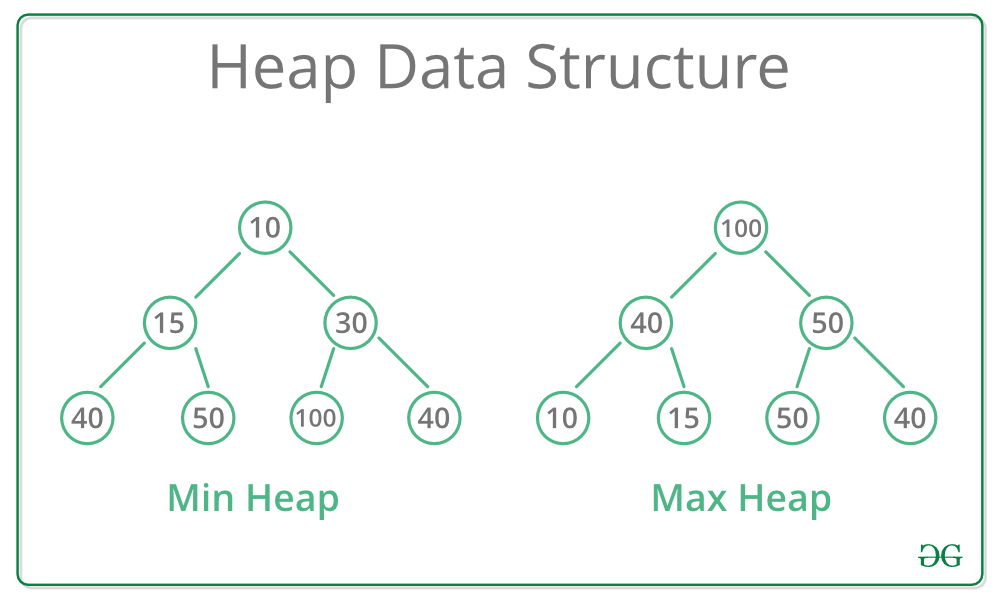
\includegraphics[width=0.75\linewidth]{images/min-max-heap.png}
                    \caption{Beispiele von Min- und Max-Heap\\\cite{EZ:Web60}}
                    \label{fig:min-max-heap}
                \end{figure}
                
                Da Min-Heaps im Zusammenhang mit Pathfinding jedoch eine schlechtere Performance aufweisen, wird hier die von Keith Schwarz implementierte \lstinline{FibonacciHeap}-Klasse verwendet. Die Struktur eines solchen Heaps ist in \abb{fig:fibonacci-heap} visualisiert. Ein Fibonacci-Heap besteht aus einer Liste von mehrerer Bäume. Dabei kann jeder Baum auch nur ein einziges Element sein. Werden Operationen wie \lstinline{insert} oder \lstinline{decreaseKey} nur selten aufgerufen, so wäre eine andere Datenstruktur wie \zb ein binärer Heap wahrscheinlich effizienter. Hier wird jedoch (WAHRSCHEIUNLICH) bei jeder Iteration \lstinline{insert} aufgerufen, . \cite{EZ:Web53, EZ:Web56}.  % TODO: mehr zur Implementierung
                
                \begin{figure}
                    \centering
                    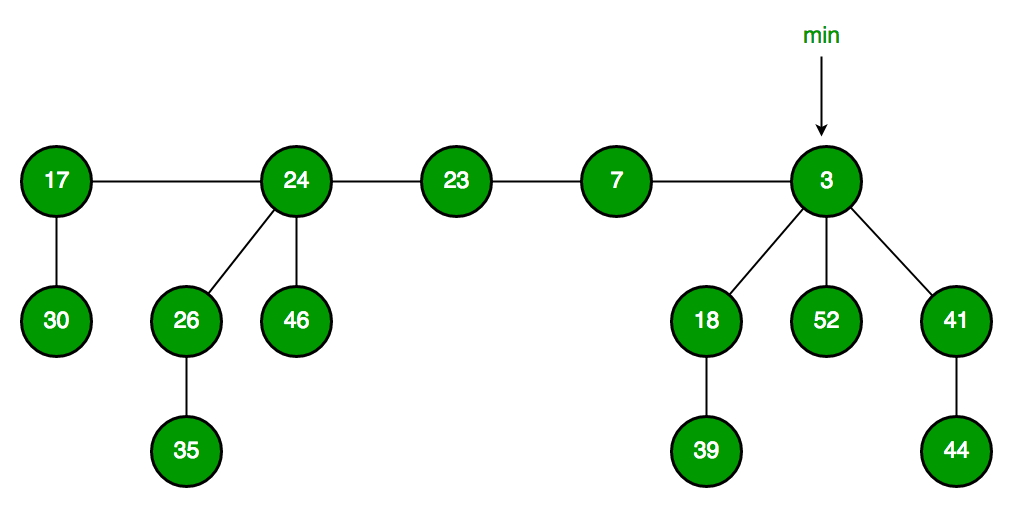
\includegraphics[width=0.75\linewidth]{images/fibonacci-heap.png}
                    \caption{Struktur eines Fibonacci-Heaps\\\cite{EZ:Web54}}
                    \label{fig:fibonacci-heap}
                \end{figure}

                Würde man in \lil{lst:abstract-befs} anstatt eines Fibonacci-Heaps eine Java-\lstinline{PriorityQueue} verwenden, so könnte die Initialisierung wie in \lil{lst:priority-queue} aussehen. Der übergebene \lstinline{Comparator} sorgt dafür, dass die Priorität eines eingefügten Knotens $n$ anhand von $f(n)$, also von der Summe von $g(n)$ und $h(n)$, bestimmt wird. Gilt $f(n_1) = f(n_2)$ für zwei Knoten $n_1$ und $n_2$, so hängt die Priorität ausschließlich von $h(n)$ ab.
    
                \begin{lstlisting}[caption=Priority-Queue mit Comparator für Best-first search, label=lst:priority-queue]
open = new PriorityQueue<>(
        Comparator.<T>comparingDouble(
                vertex -> g(vertex) + h(vertex, endCondition)
        )
        .thenComparingDouble(
                vertex -> h(vertex, endCondition)
        )
);
                \end{lstlisting}

                Mithilfe der Closed-List kann festgestellt werden, ob ein Knoten bereits besucht wurde und die aktuelle Iteration übersprungen werden, wenn das der Fall ist. Theoretisch wäre diese aber gar nicht unbedingt notwendig, würde man nämlich beim Aktualisieren der Priorität eines Knotens dafür sorgen, dass er an seine designierte Position verschoben wird, anstatt ihn neu einzufügen, und würde man eine \emph{monotone} Heuristik verwenden (\skpt{astar}), so wäre garantiert, dass kein Knoten öfter als einmal besucht wird, da kein Knoten mehrfach in der Open-List vorkommen könnte, und gleichzeitig würde man sogar Speicherplatz sparen. Das könnte in etwa wie in \lil{lst:open-decrease-key} aussehen, wobei \lstinline{entries} eine \lstinline{Map<T, FibonacciHeap.Entry<T>>} ist, welche jedem Knoten eine Referenz auf seinen Eintrag im Fibonacci-Heap zuordnet.
             
                \begin{lstlisting}[caption=Aktualisierung der Prioritäten ohne Knoten mehrfach einzufügen, label=lst:open-decrease-key]
if (entries.containsKey(neighbor)) {
    open.decreaseKey(entries.get(neighbor), tentativeG + heuristic);
} else {
    entries.put(neighbor, open.enqueue(neighbor, tentativeG + heuristic));
}
                \end{lstlisting}

                Die \lstinline{decreaseKey}-Operation hat hier die Aufgabe, die Priorität auf einen niedrigeren Wert zu ändern, und diese somit zu erhöhen. Den Wert selbst zu erhöhen wäre nicht möglich, da sonst eine Exception geworfen werden würde, \slil{lst:decrease-key}. Da \lstinline{decreaseKey} performancemäßig jedoch ziemlich teuer ist, wird hier ein einfaches \lstinline{open.enqueue(neighbor, tentativeG + heuristic)} bevorzugt, obwohl die Priorität so nur von $f(n)$ abhängt und Knoten mit demselben $f(n)$ untereinander keine bestimmte Ordnung haben. Stattdessen wird bei jeder Iteration überprüft, ob der aktuelle Knoten bereits besucht wurde und diese übersprungen, falls das der Fall ist. Zusätzlich werden mit der Zeile \lstinline{.filter(entry -> !hasVisited(entry.getKey()))} nur die Nachbarn herausgefiltert, die noch nicht besucht wurden, um die Anzahl zu überspringender Iterationen möglichst gering zu halten.

                \begin{lstlisting}[caption=decreaseKey-Methode aus \texttt{FibonacciHeap.java}, label=lst:decrease-key]
public void decreaseKey(Entry<T> entry, double newPriority) {
    checkPriority(newPriority);
    if (newPriority > entry.mPriority)
        throw new IllegalArgumentException("New priority exceeds old.");

    /* Forward this to a helper function. */
    decreaseKeyUnchecked(entry, newPriority);
}
                \end{lstlisting}

                Hierbei stellt \lstinline{checkPriority} sicher, dass die Priorität nicht auf \lstinline{Double.NaN} gesetzt werden kann, \slil{lst:check-priority}.

                \begin{lstlisting}[caption=checkPriority-Methode aus \texttt{FibonacciHeap.java}, label=lst:check-priority]
private void checkPriority(double priority) {
    if (Double.isNaN(priority))
        throw new IllegalArgumentException(priority + " is invalid.");
}
                \end{lstlisting}

                \begin{table}
                    \centering
                    \begin{tabular}{|l|l|l|} \hline
                        \textbf{Operation} & \textbf{Min-Heap} & \textbf{Fibonacci-Heap}\\ \hline
                        insert & $\bigO(\log n)$& $\bigO(1)$\\
                        getMin & $\bigO(1)$& $\bigO(1)$\\
                        extractMin & $\bigO(\log n)$ & $\bigO(\log n)^{*}$\\
                        decreaseKey & $\bigO(\log n)$ & $\bigO(1)^{*}$\\
                        remove & $\bigO(\log n)$ & $\bigO(\log n)^{*}$\\
                        merge& $\bigO(m \cdot \log(n+m))$ & $\bigO(1)$\\ \hline
                    \end{tabular}
                    \caption{Vergleich der Zeitkomplexitäten des Min- und Fibonacci-Heaps\\\cite{EZ:Web55}}
                    \label{tab:heap-time-complexities}
                \end{table}

            
            \subsubsection{Dijkstra-Algorithmus}
    
                \begin{quote}
                    \textit{What is the shortest way to travel from Rotterdam to Groningen, in general: from given city to given city. It is the algorithm for the shortest path, which I designed in about twenty minutes. One morning I was shopping in Amsterdam with my young fiancée, and tired, we sat down on the café terrace to drink a cup of coffee and I was just thinking about whether I could do this, and I then designed the algorithm for the shortest path. As I said, it was a twenty-minute invention. In fact, it was published in '59, three years later. The publication is still readable, it is, in fact, quite nice. One of the reasons that it is so nice was that I designed it without pencil and paper. I learned later that one of the advantages of designing without pencil and paper is that you are almost forced to avoid all avoidable complexities. Eventually, that algorithm became to my great amazement, one of the cornerstones of my fame.} \cite[Edsger W. Dijkstra, 2001]{EZ:Web47}
                \end{quote}
    
                Der Algorithmus von Dijkstra wurde im Jahr 1956 von Edsger W. Dijkstra entworfen und drei Jahre später veröffentlicht. Er findet in vielen verschiedenen Bereichen Anwendung, und das nicht nur bei der Navigation im Straßenverkehr, sondern zum Beispiel auch bei Routing-Protokollen für Computernetzwerke. Die zwei bekanntesten sind OSPF\footnote{Open Shortest Path First} und IS-IS\footnote{Intermediate System to Intermediate System}, welche auf dem Dijkstra-Algorithmus aufbauen. \cite{EZ:Web48, EZ:Web49}
    
                Genau genommen ist der Dijkstra-Algorithmus ein Sonderfall von A* und somit auch der allgemeinen Bestensuchen. Dijkstra ist hierbei ein Sonderfall, da immer $h(n) = 0$ und somit $f(n) = g(n)$ gilt, es wird also nur die Distanz zum Startknoten zur Bewertung miteinbezogen, die Entfernung zum Endknoten spielt somit keine Rolle. Ein weiteres wichtiges Detail des Dijkstra-Algorithmus ist, dass er normalerweise nicht nur den kürzesten Pfad zwischen zwei Knoten findet, sondern zu allen Knoten im Graphen von einem bestimmten Startpunkt aus. Um seine Effizienz zu verbessern, kann er jedoch modifiziert werden, sodass die Suche beendet wird, sobald er am Zielknoten angelangt ist bzw. die Endbedingung erreicht wurde. \cite{EZ:Web08, EZ:Web51, EZ:Web52}
                
                Die konkrete Implementierung des Dijkstra-Algorithmus ist in \lil{lst:dijkstra} veranschaulicht. Die Klasse \lstinline{Dijkstra} erbt von \lstinline{AbstractBestFirstSearch} und implementiert \lstinline{g(T vertex, Map<T, Double> distances)} so,  dass immer die Distanz des übergebenen Knotens zum Startpunkt zurückgegeben wird, bzw. $\infty$, falls diese noch nicht bekannt ist. Die Heuristik-Funktion \lstinline{h(T vertex, EndCondition<T> endCondition)} gibt hier immer den Wert $0$ zurück.
                
                Wie bereits in \kpt{befs} erwähnt, wäre es mit dem Einsatz einer monotonen Heuristik nicht unbedingt erforderlich, eine Liste von bereits besuchten Knoten zu führen, um sicherzustellen, dass der Algorithmus korrekt funktioniert und keine Knoten mehr als einmal besucht werden. Dieses Kriterium wird vom Dijkstra-Algorithmus immer erfüllt, da dieser eine implizite Heuristik von $h(n) = 0$ verwendet, welche somit monoton ist. Dass nun kein Knoten mehrfach besucht wird, wird von zwei Eigenschaften gewährleistet, wobei die zweite von der ersten impliziert wird:
                
                \begin{enumerate}
                    \item \textbf{Priorisierung kürzerer Pfade:} Der verwendete Fibonacci-Heap stellt aufgrund seiner Priority-Queue-Eigenschaften sicher, dass immer der Knoten mit dem aktuell kürzesten bekannten Pfad vom Startknoten aus besucht wird. So werden alle kürzeren Pfade vor längeren erkundet und es ist ausgeschlossen, dass ein Knoten auf einem längeren Umweg erneut besucht wird, da der Pfad dazu kürzer sein müsste. \cite{EZ:Web50}
                
                    \item \textbf{Monotonie der Distanzen:} Da die Entfernung vom Startknoten beim Verfolgen eines Pfades immer um die Gewichtungen der traversierten Kanten erhöht wird, kann die Distanz vom Startknoten zum aktuellen Knoten niemals kleiner sein als die Distanz zum Vorgängerknoten. Auch der Vorgängerknoten wird daher, obwohl er in Digraphen manchmal bzw. in ungerichteten Graphen immer Nachbar des aktuellen Knotens ist, nie mehr als einmal besucht werden, da er bereits auf einem kürzeren Pfad erreicht wurde.
                \end{enumerate}
    
                \lstinputlisting[
                    caption=Dijkstra-Algorithmus in Java,
                    label=lst:dijkstra
                ]{sources/Dijkstra.java}
                
            \subsubsection{A*-Algorithmus} \label{astar}
    
                A* ist ebenfalls ein Algorithmus aus der Klasse der BeFS\footnote{Best-first search (nicht zu verwechseln mit Breadth-first search)}-Algorithmen. Im Gegensatz zum Dijkstra-Algorithmus, bei dem immer $h(n) = 0$ gilt, spielt die Heuristik $h(n)$ hier jedoch eine wichtige Rolle.
                
                Eine Implementierung von A* ist in \lil{lst:astar} zu sehen. Die Vererbungshierarchie von \lstinline{AStar} ist von der von \lstinline{ArrayList} inspiriert. Die konkrete Klasse\lstinline{AStar} erbt von der abstrakten Klasse \lstinline{AbstractBestFirstSearch} und implementiert somit die zwei Kostenfunktionen $g$ und $h$. Die Methode \lstinline{g(T vertex, Map<T, Double> distances)} ist wie bei Dijkstra implementiert und \lstinline{h(T vertex, EndCondition<T> endCondition)} gibt den Wert der an den Konstruktor von \lstinline{AStar} übergebenen und auf die Parameter angewendeten \lstinline{Heuristic<T> heuristic} zurück.
                
                \lstinputlisting[
                    caption=A*-Algorithmus in Java,
                    label=lst:astar
                ]{sources/AStar.java}
                
                Das Interface \lstinline{Heuristic} aus \lil{lst:heuristic} ist ein \lstinline{FunctionalInterface}, welches von \lstinline{ToDoubleBiFunction<T, EndCondition<T>>} erbt. Es wird ein \lstinline{FunctionalInterface} verwendet, damit die \lstinline{h}-Methode und somit auch die \lstinline{AStar}-Klasse nicht abstrakt sein muss, und \lstinline{h} dadurch nicht jedes Mal bei der Verwendung einer neuen Heuristik neu implementiert werden muss, sondern einfach als Konstruktorparameter übergeben werden kann. \cite{EZ:Web08, EZ:Web18}
                
                \lstinputlisting[
                    caption=\texttt{Heuristic.java},
                    label=lst:heuristic
                ]{sources/Heuristic.java}

                Damit A* garantiert den optimalen Pfad finden kann, muss die Heuristik \emph{zulässig} (englisch \emph{admissible}) sein. Das ist sie dann und nur dann, wenn die von ihr geschätzte Distanz $h(n)$ vom aktuellen Knoten zum Endknoten nie die tatsächliche Mindestdistanz überschreitet. Ist die Zulässigkeit der verwendeten Heuristik nicht gegeben, so ist es besser, einen anderen Algorithmus zu verwenden, wie \zb Dijkstra, da dieser eine monotone Heuristik von $h(n) = 0$ verwendet.
                
                Damit eine Heuristik als \emph{monoton} gilt, muss zusätzlich
                
                    \[\forall n \in V: h(n) \leq h(n') + w(n, n')\]
                
                gelten. Der Wert der Heuristik muss also für jeden Knoten $n$ höchstens so groß sein wie das Maximum der Heuristik-Werte all seiner Nachbarn $n'$ plus dem Kantengewicht zwischen $n$ und $n'$. Anders ausgedrückt darf der Wert der Heuristik für keinen Knoten $n$ zu seinen Nachbarknoten $n'$ um mehr als die Gewichtung der Kante zwischen diesen sinken. Monotone bzw. \emph{konsistente} Heuristiken sind immer zulässig, umgekehrt ist dies jedoch nicht unbedingt der Fall. Verwendet A* eine monotone Heuristik, ist sichergestellt, dass jeder Knoten nur einmal besucht werden muss, da ein Knoten so erst dann besucht wird, wenn der kürzeste Pfad zu ihm gefunden wurde. \cite{EZ:Web18, EZ:Web57}

        \subsection{Bidirektionale Bestensuche} \label{bidi-befs}
        
            Die bidirektionale Bestensuche, welche auch als \emph{Meet In The Middle}-Algorithmus bezeichnet wird, ist eine Erweiterung der normalen, unidirektionalen Bestensuche. Anstatt einer einfachen Suche, die terminiert, sobald sie einen bzw. den Knoten gefunden hat, der die Endbedingung erfüllt, werden hier zwei Suchen gleichzeitig verwendet. Gleichzeitig jedoch nicht im Sinne von parallel, sondern zwischen den beiden Suchen abwechselnd. Die erste ist hierbei die \emph{Vorwärtssuche}, die wie gewohnt von Anfang bis Ende sucht. Die zweite, die \emph{Rückwärtssuche}, beginnt ihre Suche nun aber beim Endknoten und sucht in Richtung Startknoten. Das bedeutet, dass für das Funktionieren solch einer bidirektionalen Suche die Endbedingung dieser via \lstinline{EndCondition::endAt} erzeugt werden muss, da der Endknoten bei einer Erzeugung via \lstinline{EndCondition::endIf} nicht im Vorhinein bekannt wäre. Treffen die beiden Suchen aufeinander, wird der Pfad vom Startknoten zum überlappenden Knoten berechnet, woraufhin dieser Pfad mit dem vom überlappenden Knoten zum Endpunkt verschmolzen wird. Deshalb wird die bidirektionale Suche auch als \emph{Meet In The Middle}-Algorithmus bezeichnet, da die beiden Suchen in der Mitte des gesamten Pfades aufeinandertreffen, wenn der Graph symmetrisch ist. In \abb{fig:bidi} ist der konzeptionelle Unterschied zwischen bi- und unidirektionalen Suchen visualisiert.
            
            \begin{figure}
                \centering
                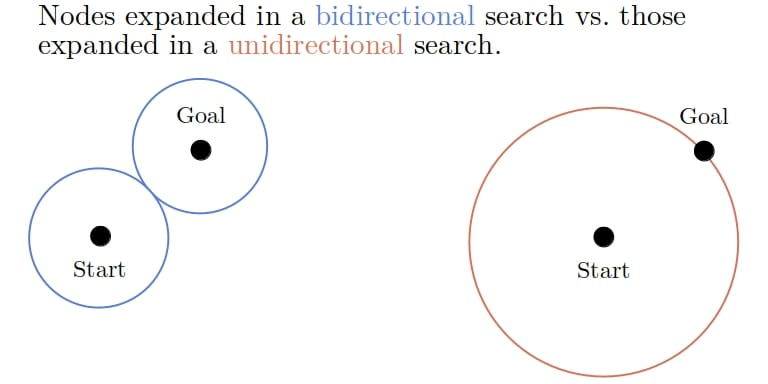
\includegraphics[width=0.6\linewidth]{images/bidi.png}
                \caption{Die Idee hinter der bidirektionalen Suche\\\cite{EZ:Web62}}
                \label{fig:bidi}
            \end{figure}
            
            Es stellt sich die Frage, welche Vorteile diese bidirektionale Art der Erkundung bietet, sogar ohne Multithreading einzusetzen. Diese kommen erst richtig zum Vorschein, wenn man den Algorithmus auf Graphen anwendet, bei denen die Anzahl erkundeter Knoten exponentiell wächst, wenn man auf ihnen eine Breitensuche ausführt. Ein Beispiel für solch einen Graphen ist der des 15-Puzzles, welches in \kpt{15-puzzle} näher erklärt wird. Dort ist die Anzahl der Knoten bei einer Erkundungstiefe von $n$ für kleine $n$ annähernd $4^n$, wobei die tatsächliche Anzahl $4^n$ aber nie überschreitet. Sucht man von nur einer Seite aus, so müsste man für einen Endknoten, der nur $20$ Schritte entfernt liegt, schon ca. $4^{20} \approx 10^{12}$ Knoten erkunden. Sucht man nun aber vom Start- zum Endknoten und umgekehrt, so muss jede der beiden Suchen nur mehr ca. $4^{10} \approx 10^6$ Knoten erkunden, also insgesamt ca. $2 \cdot 4^{10} = 2^{21} = \approx 2 \cdot 10^6$. Generell kann man also sagen, dass die bidirektionale Bestensuche die Anzahl der zu erkundenden Knoten von $m$ auf ungefähr $2 \sqrt{m}$, bzw. von $k^n$ auf ungefähr $2k^{n/2}$ reduziert, wobei $k$ die Basis der Exponentialfunktion $k^n$ ist, die die Entwicklung der Anzahl der besuchten Knoten beschreibt, wenn man auf einem Graphen eine Breitensuche mit einer maximalen Tiefe von $n$ durchführt. Eine Implementierung der bidirektionalen Bestensuche ist in \lil{lst:bidi-befs} zu sehen.

            % TODO: es KANN mit Bestensuchen wegen g(n) garantiert werden, bei meiner Impl aber NICHT
            Natürlich könnten andere Pathfinding-Algorithmen als nur Bestensuchen ebenso für bidirektionale Suchen verwendet werden, jedoch wäre dann nicht garantiert, dass sie den optimalen Pfad finden. Beispielsweise bei DFS würde das Zusammentreffen der zwei Suchen noch lange nicht bedeuten, dass sie gemeinsam den kürzesten bilden. Bei Bestensuchen ist das jedoch der Fall, da diese erst dann einen Knoten besuchen, wenn alle näheren Knoten bereits besucht wurden. Fertig implementierte Algorithmen sind unter anderem BHPA\footnote{Bidirectional Heuristic Path Algorithm}, BHFFA\footnote{Bidirectional Heuristic Front-to-Front Algorithm} und BHFFA2\footnote{BHFFA Again}. \cite{EZ:Web58, EZ:Web62, EZ:Web63, EZ:Web64}

            % TODO: fix && line break
            \lstinputlisting[
                caption=\texttt{BidiBestFirstSearch.java},
                label=lst:bidi-befs
            ]{sources/BidiBestFirstSearch.java}

    \section{Vergleich und Evaluation der Algorithmen}

        \subsection{Hilfsklassen}

            \subsubsection{Pathfinder}

                Damit man nicht bei jeder Pfadberechnung denselben Graphen und Algorithmus als Parameter übergeben muss, gibt es die generische Klasse \lstinline{Pathfinder<T>}. Sie besitzt zwei Instanzvariablen, den \lstinline{Graph<T> graph} und den \lstinline{PathfindingAlgorithm<T> algorithm}. Die Implementierung folgt somit dem Strategy-Pattern. Will man die Methoden \lstinline{findAnyPath} oder \lstinline{findShortestPath} am an den Konstruktor von \lstinline{Pathfinder} übergebenen Graphen anwenden, müssen jetzt nur mehr Start- und Zielknoten übergeben werden, da immer der gespeicherte Graph verwendet wird. Sowohl der \lstinline{Graph<T> graph} als auch der \lstinline{PathfindingAlgorithm<T> algorithm} haben Getter und Setter, beide Variablen können also im Nachhinein noch verändert werden, falls nötig.
        
                \lstinputlisting[
                    caption=\texttt{Pathfinder.java},
                    label=lst:pathfinder
                ]{sources/Pathfinder.java}
        
                Da die Klasse \lstinline{Pathfinder<T>} generisch ist, reicht es aus, den Typ \lstinline{T} nur ein einziges Mal zu spezifizieren, in diesem Fall bei der Erzeugung des Graphen, \slil{lst:type-inference}. Der Typ \lstinline{T} des \lstinline{Pathfinder<T>} kann hier durch Typinferenz bestimmt werden. Dasselbe gilt für den \lstinline{PathfindingAlgorithm<T>}, hier \lstinline{BreadthFirstSearch<T>}, \skpt{bfs}, da er erst bei der Übergabe der Konstruktorparameter erzeugt wird. Als Beispiel wird hier der Graph aus \abb{fig:abcd} verwendet. Das Print-Statement am Ende gibt wie erwartet den kürzesten Pfad von A zu D, \lstinline{[A, B, D]}, aus.
        
                \begin{lstlisting}[caption=Typinferenz, label=lst:type-inference]
    var graph = new FlexibleGraph<Character>();
    graph.addEdge('A', 'B');
    graph.addEdge('B', 'C');
    graph.addEdge('C', 'D');
    graph.addEdge('B', 'D');
    
    var finder = new Pathfinder<>(graph, new BreadthFirstSearch<>());
    System.out.println(finder.findShortestPath('A', EndCondition.endAt('D')));
                \end{lstlisting}
        
                \begin{figure}
                    \centering
                    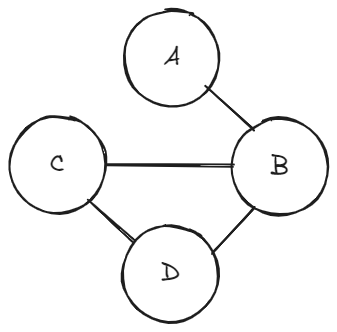
\includegraphics[width=0.5\linewidth]{images/abcd.png}
                    \caption{Graph mit zwei unterschiedlich langen Pfaden von A zu D}
                    \label{fig:abcd}
                \end{figure}
        
        \subsection{Benchmarking}

            Mithilfe der Python-Library \emph{pandas} werden die in einer CSV\footnote{Comma-separated values}-Datei gespeicherten Daten in einen DataFrame umgewandelt und . % TODO
            
            \subsubsection{Undirected ModifiableGraphRandomizer}

                In \abb{fig:corr} sind die Korrelationen zwischen den verschiedenen aufgezeichneten Spalten in einer Heatmap visualisiert. Anstatt der defaultmäßigen Pearson- werden hier die Spearman-Korrelationskoeffizienten berechnet, da die Kriterien für das Erkennen von Korrelationen so um einiges lockerer sind. Diese müssen bei Spearman nicht linear sein, sondern nur monoton. Da kein in dieser Arbeit beschriebener Pathfinding-Algorithmus eine lineare Zeitkomplexität hat, ist das von großem Vorteil. Die Spalten haben folgende Bedeutungen:

                \begin{itemize}
                    \item \textbf{Path Present:} Ob ein Pfad gefunden wurde, oder nicht
                    
                    \item \textbf{Path Length:} Die Anzahl der Knoten im Pfad, der gefunden wurde
                    
                    \item \textbf{Path Weight:} Die Summe der Gewichtungen der Kanten, die der gefundene Pfad überquert
                    
                    \item \textbf{Duration (µs):} Die Zeit in Mikrosekunden, die es gedauert hat, bis der Algorithmus den Pfad gefunden hat
                    
                    \item \textbf{Visited Vertices:} Die Anzahl an Knoten, die vom jeweiligen Algorithmus besucht wurden, um den Pfad zu finden
                    
                    \item \textbf{Average Degree:} Die durchschnittliche Nachbaranzahl jedes Knotens des Graphen, in dem der Algorithmus ausgeführt wurde

                    \item \textbf{Average Path Degree:} Die durchschnittliche Nachbaranzahl jedes Knotens des Pfades, der gefunden wurde
                \end{itemize}

                \begin{figure}
                    \centering
                    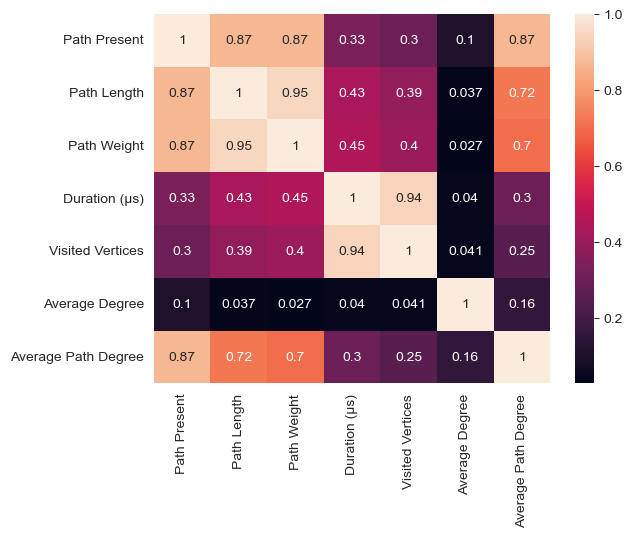
\includegraphics[width=0.75\linewidth]{images/plots/modifiable/1000/1000/1000/spf/shortest/corr.png}
                    \caption{Die Korrelationen zwischen den Spalten}
                    \label{fig:corr}
                \end{figure}

                Man kann aus der Grafik einige interessante Zusammenhänge erkennen. Die Zeitdauer, bis ein Pfad gefunden wurde, korreliert mit einem Koeffizienten von $0.94$ nahezu vollständig mit der Anzahl an besuchten Knoten.

                % TODO erklären
                % TODO: mehrere plots nebeneindaner?
                Da die Tiefensuche nicht für die Berechnung kürzester Pfade geeignet ist und somit eine Ewigkeit braucht, um zu terminieren, kommt diese nicht im folgenden \lstinline{findShortestPath}-Benchmark vor. Die rekursive Variante ist nochmal um Größenordnungen langsamer, daher wird diese erst recht nicht miteinbezogen.

                BFS am kleinsten -> optimiert Länge (assumed weights immer 1)
                BidiBeFS nicht perfekt % TODO: (auch oben im zugehören Kapitel erwähnen)

                \begin{figure}
                    \centering
                    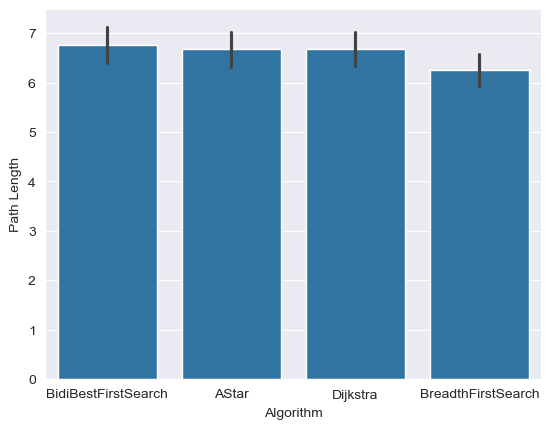
\includegraphics[width=0.5\linewidth]{images/plots/modifiable/1000/1000/1000/spf/shortest/algo_length.png}
                    \caption{Enter Caption}
                    \label{fig:enter-label1}
                \end{figure}

                BFS am größten -> vernachlässigt tatsächliche Gewichtungen

                \begin{figure}
                    \centering
                    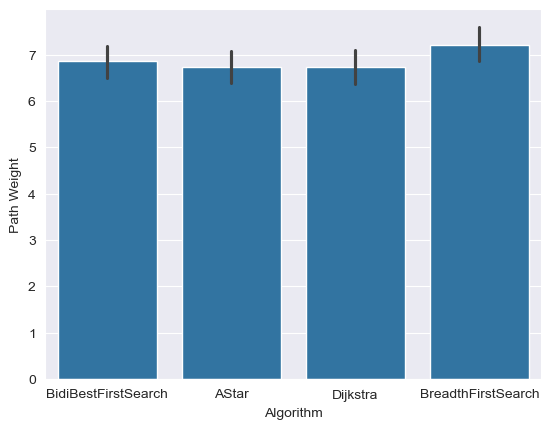
\includegraphics[width=0.5\linewidth]{images/plots/modifiable/1000/1000/1000/spf/shortest/algo_weight.png}
                    \caption{Enter Caption}
                    \label{fig:enter-label5}
                \end{figure}

                \begin{figure}
                    \centering
                    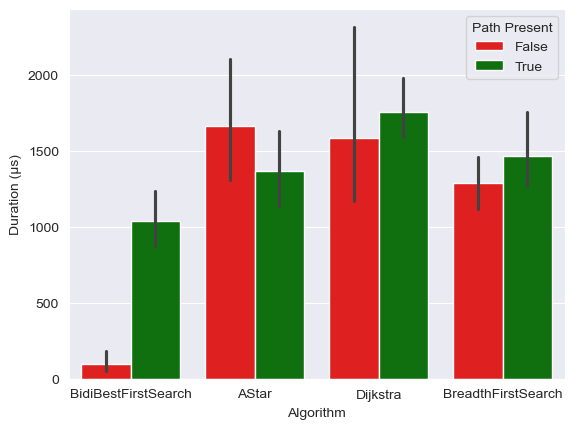
\includegraphics[width=0.5\linewidth]{images/plots/modifiable/1000/1000/1000/spf/shortest/algo_duration.png}
                    \caption{Enter Caption}
                    \label{fig:enter-label6}
                \end{figure}

                \begin{figure}
                    \centering
                    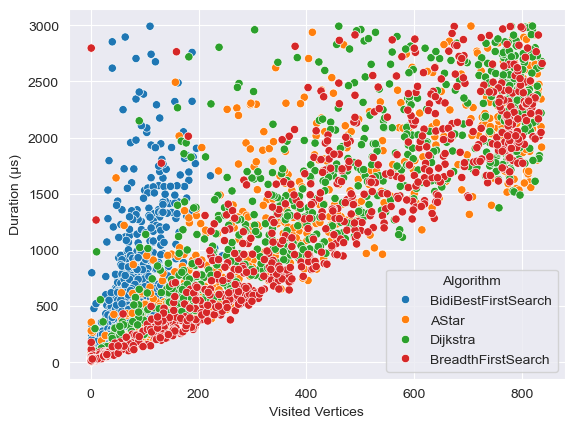
\includegraphics[width=0.5\linewidth]{images/plots/modifiable/1000/1000/1000/spf/shortest/vertices_duration.png}
                    \caption{Enter Caption}
                    \label{fig:enter-label4}
                \end{figure}

                Im folgenden \lstinline{findAnyPath}-Benchmark ist die iterative Variante der Tiefensuche inkludiert. Sogar mit dem Finden irgendeines Pfades auf nur zehn zufälligen Graphen war die rekursive Variante nach acht Stunden immer noch nicht fertig, während alle anderen Algorithmen, sogar die iterative Tiefensuche, nach nur wenigen Millisekunden bereits $1000$ Graphen geschafft haben. % TODO: mehr plots (width von barplots anpassen, schaut gacksi aus...)

                \begin{figure}
                    \centering
                    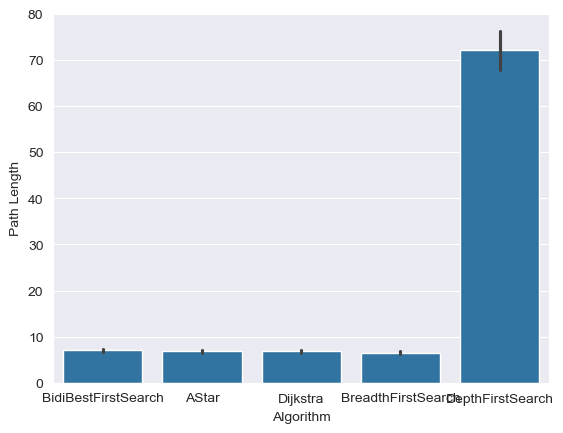
\includegraphics[width=0.5\linewidth]{images/plots/modifiable/1000/1000/1000/iterative/any/algo_length.png}
                    \caption{Enter Caption}
                    \label{fig:enter-label3}
                \end{figure}
                
                \begin{figure}
                    \centering
                    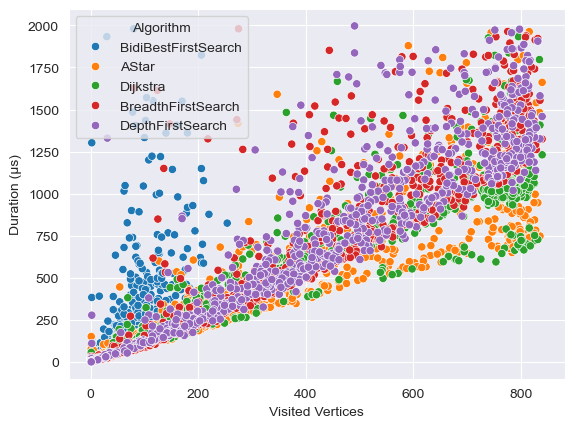
\includegraphics[width=0.5\linewidth]{images/plots/modifiable/1000/1000/1000/iterative/any/vertices_duration.png}
                    \caption{Enter Caption}
                    \label{fig:enter-label2}
                \end{figure}


            \subsubsection{Vollständiger Graph?}
                

            \subsubsection{15-Puzzle} \label{15-puzzle}

                Das 15-Puzzle ist ein klassisches Beispiel für kontraintuitive, dennoch nützliche Anwendungsfälle von Pathfinding. Es besteht aus einem Raster, welches aus vier Spalten und vier Zeilen besteht. Auf diesem sind $15$ nummerierte Tiles platziert, und um das Puzzle zu lösen, müssen diese wie in \abb{fig:15-solved} von $1$ bis $15$ aufsteigend angeordnet werden, wenn man von oben nach unten zeilenweise von links nach rechts liest.

                \begin{figure}
                    \centering
                    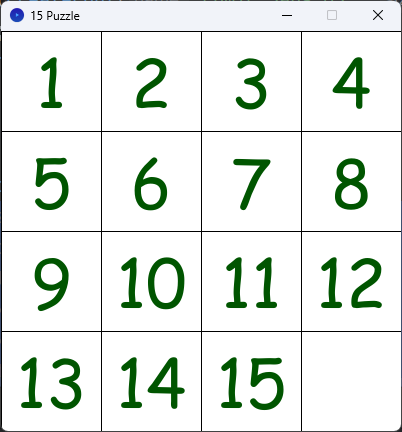
\includegraphics[width=0.5\linewidth]{images/15-puzzle-solved.png}
                    \caption{Der gelöste Zustand des 15-Puzzles}
                    \label{fig:15-solved}
                \end{figure}

                Tiles können nur verschoben werden, indem sie ihren Platz mit dem leeren Tile tauschen. Dadurch ergeben sich $16! = 2.0922789888 \cdot 10^{13}$ verschiedene mögliche Zustände. Von diesen mehr als $20$ Billionen Zuständen sind jedoch nur exakt die Hälfte lösbar, also $\frac{16!}{2} = 1.0461394944 \cdot 10^{13}$. Einer von diesen ist in \abb{fig:15-shuffled} zu sehen.
                
                \begin{figure}
                    \centering
                    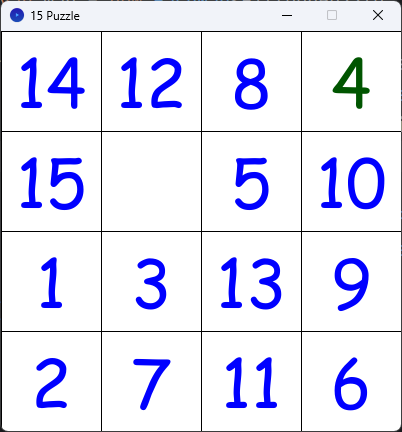
\includegraphics[width=0.5\linewidth]{images/15-puzzle-shuffled.png}
                    \caption{Ein ungelöster Zustand des 15-Puzzles}
                    \label{fig:15-shuffled}
                \end{figure}
                
                Interpretiert man nun jeden lösbaren Zustand als Knoten eines Graphen, so wird klar, dass seine Speicherung nicht so einfach funktionieren kann. Nimmt man an, dass jeder Knoten nur $32$ Bit an Speicherplatz benötigt, so bräuchte man schon $32 \cdot \frac{16!}{2}$ Bit $= 3.34764638208 \cdot 10^{14}$ Bit $= 4.1845579776 \cdot 10^{13}$ Byte $\approx 41$ Terabyte, um diesen Graphen auf einmal im RAM zu halten, was schlichtweg unmöglich ist. Zieht man nun zusätzlich in Betracht, dass jedes der $16$ Tiles ($15$ nummerierte + $1$ leeres) als $32$-Bit \lstinline{int} dargestellt wird, so erhöht sich der Speicherverbrauch nochmal auf das $16$-fache, also $16 \cdot 41.845579776$ Terabyte $\approx 670$ Terabyte, und das, ohne Objektreferenzen miteinzubeziehen. Wegen Fällen wie solchen ist \lstinline{Graph} ein Interface: damit die \lstinline{getNeighbors}-Methode beliebig implementiert werden kann. Für das 15-Puzzle existiert eine eigene \lstinline{FifteenPuzzleGraph}-Klasse, die die Methode so implementiert, dass alle Zustände zurückgegeben werden, die von dem übergebenen Zustand aus innerhalb eines Zuges erreicht werden können, \slil{lst:15-graph}. So muss der Graph nie als Ganzes abgespeichert werden, dafür müssen seine Nachbarn bei jedem \lstinline{getNeighbors}-Aufruf neu berechnet werden. \lstinline{Direction} ist hierbei ein Enum mit den $4$ Werten \lstinline{UP}, \lstinline{DOWN}, \lstinline{LEFT} und \lstinline{RIGHT}.
                
                \lstinputlisting[
                    caption=Repräsentation des 15-Puzzles als Graph,
                    label=lst:15-graph
                ]{sources/FifteenPuzzleGraph.java}
                
                Die abstrakte Klasse \lstinline{MemoizedGraph} aus \lil{lst:memoized-graph}, welche \lstinline{Graph} implementiert, sorgt dafür, dass bereits berechnete Nachbarn eines Knotens nicht bei jedem Zugriff erneut berechnet werden müssen, sondern memoisiert bzw. zwischengespeichert werden, um Rechenzeit zu ersparen. Da die Berechnung der Nachbarzustände beim 15-Puzzle performancemäßig jedoch ziemlich billig ist, hat Memoization hier sogar einen negativen Einfluss auf die Performance, weshalb \lstinline{FifteenPuzzleGraph} direkt \lstinline{Graph} implementiert, ohne einen Vererbungs-Umweg über \lstinline{MemoizedGraph} zu nehmen. \cite{EZ:Web59}

                \lstinputlisting[
                    caption=\texttt{MemoizedGraph.java},
                    label=lst:memoized-graph
                ]{sources/MemoizedGraph.java}

                % TODO: ACTUAL BENCHMARKING

                asd

            \subsubsection{Rubik's Cube}

                Ein ähnliches Problem, welches sich ebenfalls mit Pathfinding lösen lasst, ist der Zauberwürfel bzw. Rubik's Cube. Bei diesem kann ebenfalls jeder lösbare Zustand als Knoten eines Graphen interpretiert und das Rätsel auf eine ähnliche Weise gelöst werden. Beim Rubik's Cube gibt es im Gegensatz zu den maximal $4$ Nachbarzuständen des 15-Puzzles immer $18$, \sabb{fig:cube-neighbors}. Das macht das Problem zu einem viel komplexeren. Zusätzlich beträgt die Anzahl seiner möglichen Zustände nicht nur mehr als $10^{13}$ sondern über $4 \cdot 10^{19}$.
                
                \begin{figure}
                    \centering
                    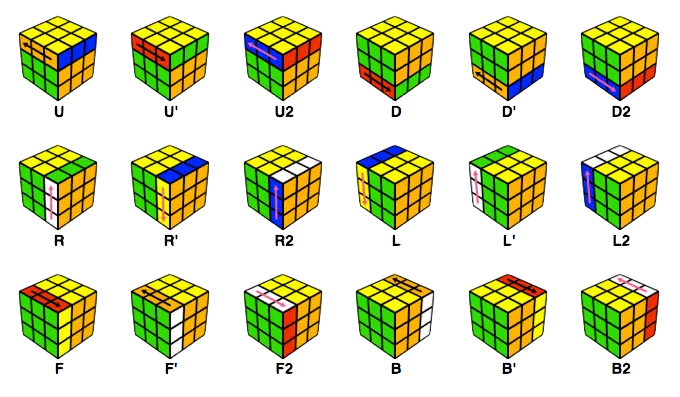
\includegraphics[width=0.75\linewidth]{images/cube-neighbors.png}
                    \caption{Die $18$ möglichen Züge beim Rubik's Cube\\\cite{EZ:Web61}}
                    \label{fig:cube-neighbors}
                \end{figure}
                
        \subsection{Zusammenfassung der Ergebnisse}

            A* am besten wenn gute Heuristik verfügbar, ansonsten Dijkstra o.ä.
            USW % TODO
            
            \begin{table}
                \centering
                \begin{tabular}{l|c|c}
                    Algorithmus & Vorteile & Nachteile\\
                    BFS &  &\\
                    DFS &  &\\
                    Dijkstra &  &\\
                    A* &  &\\
                    BidiBeFS &  &\\
                \end{tabular}
                \caption{Caption}
                \label{tab:pros-cons}
            \end{table}
    
    \section{Projektbezug}

        % TODO: sonst eh keiner CARLA erwähnt? (in dem Kontext)
        Das Projekt \emph{LiCAR} hat die Aufgabe, das Modellauto aus \abb{fig:car} selbstständig zwischen zwei Punkten navigieren zu lassen. Dazu muss zuerst ein Agent in einer Testumgebung trainiert werden. Bestenfalls in einer simulierten, damit keinerlei Schäden angerichtet werden können. Diese simulierte Testumgebung wird LiCAR von \emph{CARLA}, einer Verkehrs-Simulationssoftware, zur Verfügung gestellt. Für die effiziente Navigation dieses Agents ist Pathfinding zwingend notwendig. Über die Python-API von CARLA kann man die Topologie einer Map erhalten. Aus dieser kann mithilfe von NetworkX ein Graph erzeugt werden, \slil{lst:carla-graph}. In der echten Welt könnte dieser mithilfe einer zweidimensionalen Punktwolke erstellt werden, die direkt aus dem am Dach des Modellautos montierten LiDAR-Sensor ausgelesen wird. Die rohen LiDAR-Daten können dann \zb mittels SLAM\footnote{Simultaneous Localization and Mapping} zu einem Graphen konvertiert werden, auf dem sowohl in dieser Arbeit genannte als auch andere Pathfinding-Algorithmen angewandt werden können.

        \begin{lstlisting}[language=Python, caption=Erzeugung eines Graphen aus einer CARLA-Map, label=lst:carla-graph]
import carla
import math
import networkx as nx

client = carla.Client('localhost', 2000)
world = client.get_world()
topology = world.get_map().get_topology()

graph = nx.Graph()
graph.add_edges_from(topology)
        \end{lstlisting}

        NetworkX bietet auch eine Menge an vorgefertigten Methoden für Pfadberechnungen, wobei die für LiCAR mit Abstand wichtigste \lstinline{shortest_path} ist. In \lil{lst:nx} kann man sehen, wie diese Methode in der Praxis angewandt werden könnte. Ähnlicher Code wird intern von LiCAR verwendet.

        \begin{lstlisting}[language=Python, caption=Berechnung des kürzesten Pfades mittels NetworkX, label=lst:nx]
nodes = list(graph)
start = nodes[0]
end = nodes[-1]

path = nx.shortest_path(
    graph,
    source=start,
    target=end,
    weight=lambda u, v, attributes: math.hypot(
        u.transform.location.x - v.transform.location.x,
        u.transform.location.y - v.transform.location.y
    )
    method='dijkstra'
)
        \end{lstlisting}

        Standardmäßig verwendet \lstinline{shortest_path} den Dijkstra-Algorithmus, der optionale Parameter \lstinline{method} kann aber anstatt auf \lstinline{'dijkstra'} auch auf \lstinline{'bellman-ford'} gesetzt werden, damit der Bellman-Ford-Algorithmus benutzt wird. Der Hauptvorteil von Bellman-Ford gegenüber Dijkstra besteht darin, dass dieser mit negativen Kantengewichtungen umgehen kann, ist aber dafür zeitaufwendiger. Die Lambda-Expression, auf die \lstinline{weight} gesetzt wird, berechnet die euklidische Distanz zwischen zwei CARLA-Waypoints. Das ist notwendig, da \lstinline{add_edges_from} keine Gewichtungen setzt. Man bekommt die drei Parameter \lstinline{u}, \lstinline{v} und \lstinline{attributes} übergeben, wobei \lstinline{u} und \lstinline{v} den Anfangs- bzw. Endknoten der Kante darstellen, deren Gewichtung berechnet werden soll. Dabei ist \lstinline{attributes} ein \lstinline[language=Python]{dict}, welches Attribute der Kante enthält.

        \begin{figure}
            \centering
            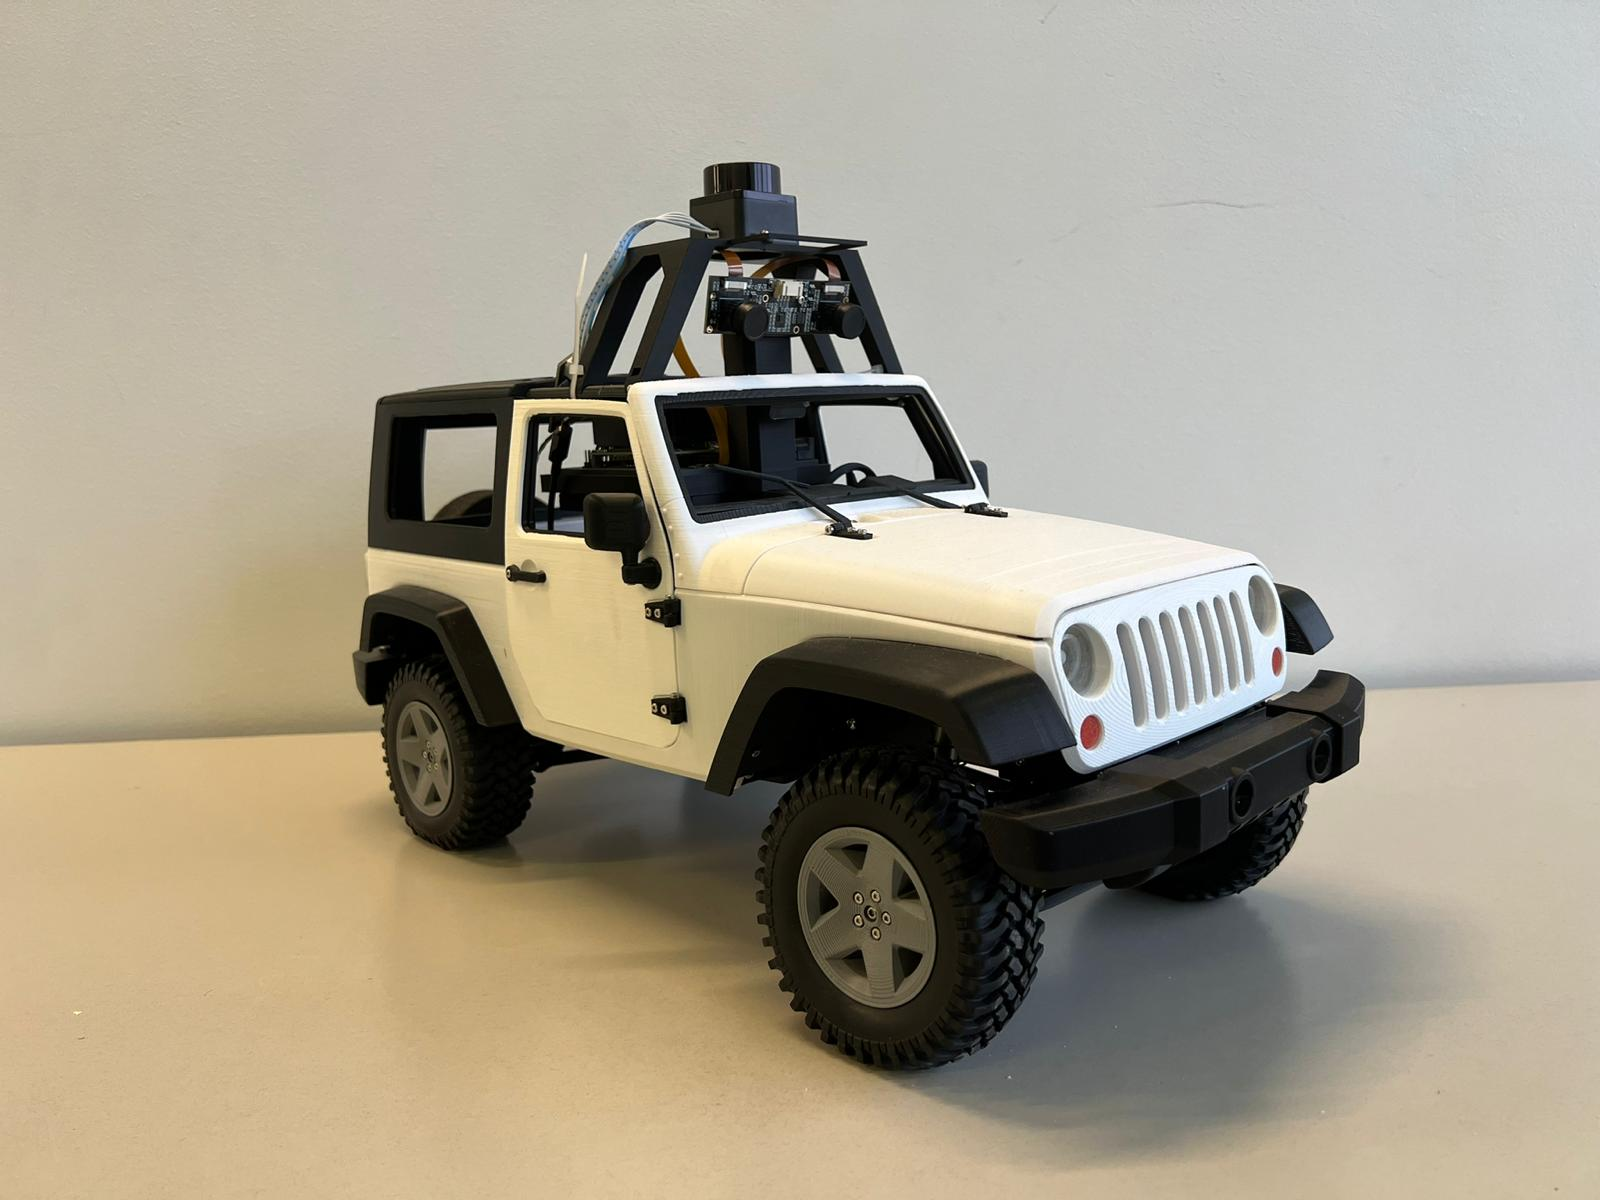
\includegraphics[width=0.5\linewidth]{images/car.jpg}
            \caption{Das von LiCAR verwendete Modellauto}
            \label{fig:car}
        \end{figure}

    \clearpage
    % \input{textparts/samples}
    % \clearpage
    
    %--------------------------------------------------------------------------
    % Anhang
    %--------------------------------------------------------------------------

    
    
    \addcontentsline{toc}{chapter}{Anhang}
    \phantomsection
    \addcontentsline{toc}{section}{Abbildungsverzeichnis}
    \listoffigures
    
    \cleardoublepage
    \phantomsection
    
    \addcontentsline{toc}{section}{Tabellenverzeichnis}
    \listoftables
    \cleardoublepage
    \phantomsection
    
    \addcontentsline{toc}{section}{Verzeichnis der Listings}
    \lstlistoflistings
    \cleardoublepage
    \phantomsection
    
    %\addcontentsline{toc}{section}{Index}
    \printindex
    \cleardoublepage
    \phantomsection
    
    \addcontentsline{toc}{section}{Literaturverzeichnis}
    %\bibliographystyle{alpha} 		 %Standardstyle
    %\bibliographystyle{dinat}		 %Style und Layout nach DIN 1502
    %\bibliography{tiger}					 %Literaturverzeichnis einfügen

    \begin{thebibliography}{999}
    
    \bibitem[EZ:Web01]{EZ:Web01}
    \href{https://www.ionos.at/digitalguide/online-marketing/web-analyse/pathfinding}{https://www.ionos.at/digitalguide/online-marketing/web-analyse/pathfinding}\\
    Pathfinding: Wegfindung in der Informatik\\
    03.11.2023
    
    \bibitem[EZ:Web02]{EZ:Web02}
    \href{https://www.geeksforgeeks.org/a-search-algorithm/}{https://www.geeksforgeeks.org/a-search-algorithm/}\\
    A*-Algorithm\\
    28.10.2023
    
    \bibitem[EZ:Web03]{EZ:Web03}
    \href{https://arxiv.org/pdf/physics/0510162.pdf}{https://arxiv.org/pdf/physics/0510162.pdf}\\
    Structural Properties of Planar Graphs of Urban Street Patterns\\
    03.11.2023
    
    \bibitem[EZ:Web04]{EZ:Web04}
    \href{https://www.baeldung.com/cs/weighted-vs-unweighted-graphs}{https://www.baeldung.com/cs/weighted-vs-unweighted-graphs}\\
    Weighted vs. Unweighted Graphs\\
    28.10.2023
    
    \bibitem[EZ:Web05]{EZ:Web05}
    \href{https://happycoding.io/tutorials/libgdx/pathfinding}{https://happycoding.io/tutorials/libgdx/pathfinding}\\
    Pathfinding\\
    04.11.2023
    
    \bibitem[EZ:Web06]{EZ:Web06}
    \href{https://studyflix.de/informatik/grundbegriffe-der-graphentheorie-1285}{https://studyflix.de/informatik/grundbegriffe-der-graphentheorie-1285}\\
    Grundbegriffe der Graphentheorie\\
    13.11.2023
    
    \bibitem[EZ:Web07]{EZ:Web07}
    \href{https://blog.viking-studios.net/wp-content/uploads/2013/04/Pathfinding-Algorithmen-in-verschiedenen-Spielegenres.pdf}{https://blog.viking-studios.net/wp-content/uploads/2013/04/Pathfinding-Algorithmen-in-verschiedenen-Spielegenres.pdf}\\
    Pathfinding-Algorithmen in verschiedenen Spielegenres\\
    14.11.2023
    
    \bibitem[EZ:Web08]{EZ:Web08}
    \href{https://yuminlee2.medium.com/a-search-algorithm-42c1a13fcf9f}{https://yuminlee2.medium.com/a-search-algorithm-42c1a13fcf9f}\\
    A* Search Algorithm\\
    14.11.2023
    
    \bibitem[EZ:Web09]{EZ:Web09}
    \href{http://gitta.info/Accessibilit/de/html/NetworkChara_learningObject1.html}{http://gitta.info/Accessibilit/de/html/NetworkChara\_learningObject1.html}\\
    Charakterisierung von Netzwerken\\
    20.11.2023
    
    \bibitem[EZ:Web10]{EZ:Web10}
    \href{https://hyperskill.org/learn/step/5645}{https://hyperskill.org/learn/step/5645}\\
    Weighted Graph\\
    14.11.2023
    
    \bibitem[EZ:Web11]{EZ:Web11}
    \href{https://mathworld.wolfram.com/GraphCycle.html}{https://mathworld.wolfram.com/GraphCycle.html}\\
    Graph Cycle\\
    20.11.2023
    
    \bibitem[EZ:Web12]{EZ:Web12}
    \href{https://www.geeksforgeeks.org/what-is-cyclic-graph/}{https://www.geeksforgeeks.org/what-is-cyclic-graph/}\\
    What is Cyclic Graph\\
    15.11.2023
    
    \bibitem[EZ:Web13]{EZ:Web13}
    \href{https://files.ifi.uzh.ch/cl/siclemat/lehre/hs07/ecl1/script/html/scriptse50.html}{https://files.ifi.uzh.ch/cl/siclemat/lehre/hs07/ecl1/script/html/scriptse50.html}\\
    Graphen\\
    16.11.2023
    
    \bibitem[EZ:Web14]{EZ:Web14}
    \href{https://mathworld.wolfram.com/CycleGraph.html}{https://mathworld.wolfram.com/CycleGraph.html}\\
    Cycle Graph\\
    20.11.2023
    
    \bibitem[EZ:Web15]{EZ:Web15}
    \href{https://www.geeksforgeeks.org/degree-of-a-cycle-graph/}{https://www.geeksforgeeks.org/degree-of-a-cycle-graph/}\\
    Degree of a Cycle Graph\\
    16.11.2023
    
    \bibitem[EZ:Web16]{EZ:Web16}
    \href{https://en.wikipedia.org/wiki/Cycle_(graph_theory)}{https://en.wikipedia.org/wiki/Cycle\_(graph\_theory)}\\
    Cycle (graph theory)\\
    16.11.2023
    
    \bibitem[EZ:Web17]{EZ:Web17}
    \href{https://de.wikipedia.org/wiki/Zyklus_(Graphentheorie)}{https://de.wikipedia.org/wiki/Zyklus\_(Graphentheorie)}\\
    Zyklus (Graphentheorie)\\
    16.11.2023
    
    \bibitem[EZ:Web18]{EZ:Web18}
    \href{https://en.wikipedia.org/wiki/A*_search_algorithm}{https://en.wikipedia.org/wiki/A*\_search\_algorithm}\\
    A* search algorithm\\
    16.11.2023
    
    \bibitem[EZ:Web19]{EZ:Web19}
    \href{https://de.wikipedia.org/wiki/Bipartiter_Graph}{https://de.wikipedia.org/wiki/Bipartiter\_Graph}\\
    Bipartiter Graph\\
    20.11.2023
    
    \bibitem[EZ:Web20]{EZ:Web20}
    \href{https://de.wikipedia.org/wiki/Gerichteter_Graph}{https://de.wikipedia.org/wiki/Gerichteter\_Graph}\\
    Gerichteter Graph\\
    20.11.2023
    
    \bibitem[EZ:Web21]{EZ:Web21}
    \href{https://www.geeksforgeeks.org/implementing-generic-graph-in-java}{https://www.geeksforgeeks.org/implementing-generic-graph-in-java}\\
    Implementing Generic Graph in Java\\
    20.11.2023
    
    \bibitem[EZ:Web22]{EZ:Web22}
    \href{https://de.wikipedia.org/wiki/Kantengewichteter_Graph}{https://de.wikipedia.org/wiki/Kantengewichteter\_Graph}\\
    Kantengewichteter Graph\\
    24.11.2023
    
    \bibitem[EZ:Web23]{EZ:Web23}
    \href{https://www.mathe-online.at/symbole.html}{https://www.mathe-online.at/symbole.html}\\
    Mathematische Symbole und Abkürzungen\\
    24.11.2023

    \bibitem[EZ:Web24]{EZ:Web24}
    \href{https://www.mathsisfun.com/sets/symbols.html}{https://www.mathsisfun.com/sets/symbols.html}\\
    Set Symbols\\
    24.11.2023

    \bibitem[EZ:Web25]{EZ:Web25}
    \href{https://en.wikipedia.org/wiki/Graph_(discrete_mathematics)}{https://en.wikipedia.org/wiki/Graph\_(discrete\_mathematics)}\\
    Graph (discrete mathematics)\\
    24.11.2023

    \bibitem[EZ:Web26]{EZ:Web26}
    \href{https://de.wikipedia.org/wiki/Einfacher_Graph}{https://de.wikipedia.org/wiki/Einfacher\_Graph}\\
    Einfacher Graph\\
    24.11.2023

    \bibitem[EZ:Web27]{EZ:Web27}
    \href{https://de.wikipedia.org/wiki/Schleife_(Graphentheorie)}{https://de.wikipedia.org/wiki/Schleife\_(Graphentheorie)}\\
    Schleife (Graphentheorie)\\
    24.11.2023

    \bibitem[EZ:Web28]{EZ:Web28}
    \href{https://en.wikipedia.org/wiki/Loop_(graph_theory)}{https://en.wikipedia.org/wiki/Loop\_(graph\_theory)}\\
    Loop (graph theory)\\
    24.11.2023

    \bibitem[EZ:Web29]{EZ:Web29}
    \href{https://de.wikipedia.org/wiki/Graph_(Graphentheorie)}{https://de.wikipedia.org/wiki/Graph\_(Graphentheorie)}\\
    Graph (Graphentheorie)\\
    24.11.2023

    \bibitem[EZ:Web30]{EZ:Web30}
    \href{https://de.wikipedia.org/wiki/Idempotenz}{https://de.wikipedia.org/wiki/Idempotenz}\\
    Idempotenz\\
    27.11.2023

    \bibitem[EZ:Web31]{EZ:Web31}
    \href{https://en.wikipedia.org/wiki/Adjacency_list}{https://en.wikipedia.org/wiki/Adjacency\_list}\\
    Adjacency list\\
    27.11.2023

    \bibitem[EZ:Web32]{EZ:Web32}
    \href{https://www.scaler.com/topics/data-structures/graph-in-data-structure/}{https://www.scaler.com/topics/data-structures/graph-in-data-structure/}\\
    Graph in Data Structure\\
    27.11.2023

    \bibitem[EZ:Web33]{EZ:Web33}
    \href{https://de.wikipedia.org/wiki/Vollständiger_Graph}{https://de.wikipedia.org/wiki/Vollständiger\_Graph}\\
    Vollständiger Graph\\
    27.11.2023

    \bibitem[EZ:Web34]{EZ:Web34}
    \href{https://en.wikipedia.org/wiki/Complete_graph}{https://en.wikipedia.org/wiki/Complete\_graph}\\
    Complete graph\\
    27.11.2023

    \bibitem[EZ:Web35]{EZ:Web35}
    \href{https://de.wikipedia.org/wiki/Knotengewichteter_Graph}{https://de.wikipedia.org/wiki/Knotengewichteter\_Graph}\\
    Knotengewichteter Graph\\
    28.11.2023

    \bibitem[EZ:Web36]{EZ:Web36}
    \href{https://de.wikipedia.org/wiki/Adjazenzmatrix}{https://de.wikipedia.org/wiki/Adjazenzmatrix}\\
    Adjazenzmatrix\\
    28.11.2023

    \bibitem[EZ:Web37]{EZ:Web37}
    \href{https://en.wikipedia.org/wiki/Adjacency_matrix}{https://en.wikipedia.org/wiki/Adjacency\_matrix}\\
    Adjacency matrix\\
    28.11.2023

    \bibitem[EZ:Web38]{EZ:Web38}
    \href{https://de.wikipedia.org/wiki/Reductio_ad_absurdum}{https://de.wikipedia.org/wiki/Reductio\_ad\_absurdum}\\
    Reductio ad absurdum\\
    28.11.2023

    \bibitem[EZ:Web39]{EZ:Web39}
    \href{https://de.wikipedia.org/wiki/Kante_(Graphentheorie)}{https://de.wikipedia.org/wiki/Kante\_(Graphentheorie)}\\
    Kante (Graphentheorie)\\
    29.11.2023

    \bibitem[EZ:Web40]{EZ:Web40}
    \href{https://www.educative.io/answers/what-is-an-adjacency-list}{https://www.educative.io/answers/what-is-an-adjacency-list}\\
    What is an adjacency list?\\
    29.11.2023

    \bibitem[EZ:Web41]{EZ:Web41}
    \href{https://cseweb.ucsd.edu/~kube/cls/100/Lectures/lec11/lec11-8.html}{https://cseweb.ucsd.edu/{\textasciitilde}kube/cls/100/Lectures/lec11/lec11-8.html}\\
    Adjacency matrices\\
    29.11.2023

    \bibitem[EZ:Web42]{EZ:Web42}
    \href{https://iq.opengenus.org/adjacency-matrix/}{https://iq.opengenus.org/adjacency-matrix/}\\
    Adjacency Matrices Explained: A Representation of Graphs\\
    29.11.2023

    \bibitem[EZ:Web43]{EZ:Web43}
    \href{https://people.engr.tamu.edu/djimenez/ut/utsa/cs1723/lecture16.html}{https://people.engr.tamu.edu/djimenez/ut/utsa/cs1723/lecture16.html}\\
    Weighted Graphs\\
    29.11.2023

    \bibitem[EZ:Web44]{EZ:Web44}
    \href{https://refactoring.guru/design-patterns/builder}{https://refactoring.guru/design-patterns/builder}\\
    Builder\\
    30.11.2023

    \bibitem[EZ:Web45]{EZ:Web45}
    \href{https://networkx.org/}{https://networkx.org/}\\
    NetworkX\\
    1.12.2023 

    \bibitem[EZ:Web46]{EZ:Web46}
    \href{https://jgrapht.org/}{https://jgrapht.org/}\\
    JGraphT\\
    1.12.2023

    \bibitem[EZ:Web47]{EZ:Web47}
    \href{https://en.wikipedia.org/wiki/Dijkstra's_algorithm}{https://en.wikipedia.org/wiki/Dijkstra's\_algorithm}\\
    Dijkstra's algorithm\\
    29.01.2024

    \bibitem[EZ:Web48]{EZ:Web48}
    \href{https://de.wikipedia.org/wiki/Open_Shortest_Path_First}{https://de.wikipedia.org/wiki/Open\_Shortest\_Path\_First}\\
    Open Shortest Path First\\
    06.02.2024

    \bibitem[EZ:Web49]{EZ:Web49}
    \href{https://en.wikipedia.org/wiki/Open_Shortest_Path_First}{https://en.wikipedia.org/wiki/Open\_Shortest\_Path\_First}\\
    Open Shortest Path First\\
    06.02.2024

    \bibitem[EZ:Web50]{EZ:Web50}
    \href{https://stackoverflow.com/questions/19894509}{https://stackoverflow.com/questions/19894509}\\
    What is the purpose of the visited set in Dijkstra?\\
    15.02.2024

    \bibitem[EZ:Web51]{EZ:Web51}
    \href{https://de.wikipedia.org/wiki/Greedy-Algorithmus}{https://de.wikipedia.org/wiki/Greedy-Algorithmus}\\
    Greedy-Algorithmus\\
    15.02.2024

    \bibitem[EZ:Web52]{EZ:Web52}
    \href{https://en.wikipedia.org/wiki/Greedy_algorithm}{https://en.wikipedia.org/wiki/Greedy\_algorithm}\\
    Greedy algorithm\\
    15.02.2024

    \bibitem[EZ:Web53]{EZ:Web53}
    \href{https://keithschwarz.com/interesting/code/?dir=fibonacci-heap}{https://keithschwarz.com/interesting/code/?dir=fibonacci-heap}\\
    FibonacciHeap.java\\
    20.02.2024
    
    \bibitem[EZ:Web54]{EZ:Web54}
    \href{https://www.geeksforgeeks.org/fibonacci-heap-set-1-introduction/}{https://www.geeksforgeeks.org/fibonacci-heap-set-1-introduction/}\\
    Fibonacci Heap | Set 1 (Introduction)\\
    23.02.2024

    \bibitem[EZ:Web55]{EZ:Web55}
    \href{https://de.wikipedia.org/wiki/Fibonacci-Heap}{https://de.wikipedia.org/wiki/Fibonacci-Heap}\\
    Fibonacci-Heap\\
    23.02.2024

    \bibitem[EZ:Web56]{EZ:Web56}
    \href{https://stackoverflow.com/questions/6065710}{https://stackoverflow.com/questions/6065710}\\
    How does Java's PriorityQueue differ from a min-heap?\\
    25.02.2024

    \bibitem[EZ:Web57]{EZ:Web57}
    \href{https://de.wikipedia.org/wiki/A*-Algorithmus}{https://de.wikipedia.org/wiki/A*-Algorithmus}\\
    A*-Algorithmus\\
    27.02.2024

    \bibitem[EZ:Web58]{EZ:Web58}
    \href{https://en.wikipedia.org/wiki/Bidirectional_search}{https://en.wikipedia.org/wiki/Bidirectional\_search}\\
    Bidirectional search\\
    03.03.2024

    \bibitem[EZ:Web59]{EZ:Web59}
    \href{https://de.wikipedia.org/wiki/Memoisation}{https://de.wikipedia.org/wiki/Memoisation}\\
    Memoisation\\
    09.03.2024

    \bibitem[EZ:Web60]{EZ:Web60}
    \href{https://www.geeksforgeeks.org/heap-data-structure/}{https://www.geeksforgeeks.org/heap-data-structure/}\\
    Heap Data Structure\\
    09.03.2024

    \bibitem[EZ:Web61]{EZ:Web61}
    \href{https://medium.com/nerd-for-tech/3cb9b53f94b5}{https://medium.com/nerd-for-tech/3cb9b53f94b5}\\
    Rubik’s Cube algorithms for machines\\
    15.03.2024

    \bibitem[EZ:Web62]{EZ:Web62}
    \href{https://www.baeldung.com/cs/bidirectional-search}{https://www.baeldung.com/cs/bidirectional-search}\\
    Bidirectional Search for Path Finding\\
    15.03.2024

    \bibitem[EZ:Web63]{EZ:Web63}
    \href{https://www.youtube.com/watch?v=A60q6dcoCjw}{https://www.youtube.com/watch?v=A60q6dcoCjw}\\
    The hidden beauty of the A* algorithm\\
    15.03.2024

    \bibitem[EZ:Web64]{EZ:Web64}
    \href{https://www.youtube.com/watch?v=wL3uWO-KLUE}{https://www.youtube.com/watch?v=wL3uWO-KLUE}\\
    The hidden beauty of the A* algorithm\\
    15.03.2024
    
\end{thebibliography} 
    \cleardoublepage
    \phantomsection    
 
\end{document}